\documentclass[10pt]{beamer}

\usetheme{metropolis}
\usepackage{appendixnumberbeamer}

\usepackage{booktabs}
\usepackage[scale=2]{ccicons}
%----------------------------
\newcommand\alertitem[1]{\alert<+>{\item {#1}}}
\usepackage[lined,ruled,vlined,commentsnumbered]{algorithm2e}
\newcommand*{\MG}{\VarCal{M}}  
%To draw pictures
\usepackage{pgf}
\usetikzlibrary{arrows,automata}
\usetikzlibrary{positioning}
\usetikzlibrary{calc}
\usetikzlibrary{shapes.geometric}
\usetikzlibrary{arrows.meta}
\usetikzlibrary{decorations.pathmorphing}

\usepackage{amsthm}
\theoremstyle{plain}
\newtheorem{thm}{Theorem}
\newtheorem{lem}{Lemma}

\theoremstyle{definition}
\newtheorem{defn}{Definition}
\newtheorem{observation}{Observation}
\newcommand{\Tau}{\mathrm{T}}
\newcommand*{\Secref}[1]{Section ~{#1}}

\newcommand*{\withbot}[1]{{#1}_\bot}
\newcommand*{\Nbot}{\withbot{N}}
\newcommand*{\Pbot}{\withbot{P_0}}

\newcommand*{\Var}[1]{\ensuremath{\mathit{#1}}}
\newcommand*{\Sec}[1]{Sec.~\ref{#1}}
\newcommand*{\Alg}[1]{Algorithm~\ref{#1}}
\newcommand*{\Fig}[2][]{Fig.~\ref{#2}{#1}}

\newcommand*{\Unseen}{\Var{Unseen}}
\newcommand*{\Seen}{\Var{Seen}}
\newcommand*{\Visited}{\Var{Visited}}

\newcommand*{\Active}{\Var{active}}
\newcommand*{\Born}{\Var{born}}
\newcommand*{\Needed}{\Var{needed}}
\newcommand*{\Origins}{\Var{origins}}

\newcommand*{\RangeOfReset}{\Var{range}\_\Var{of}\_\Var{reset}}
\newcommand*{\Range}{\Var{range}}
\newcommand*{\Ranges}{\Var{Ranges}}
\newcommand*{\RangeOfClock}{\Var{range}\_\Var{of}\_\Var{clock}}
\newcommand*{\PartitionIntoASetOfGroups}
{\Var{partition}-\Var{into}-\Var{a}-\Var{set}-\Var{of}-\Var{groups}}

\newcommand*{\Ind}{\hspace{1em}}

\newcommand*{\Rel}[1]{\ensuremath{\Var{rel}_{#1}}}   % relation of being related
\newcommand*{\RelClosure}[1]{\ensuremath{\Rel{#1}^*}}       % and its closure
\newcommand*{\Relate}[2]{\ensuremath{\Var{Rel}(#1, #2)}}

%----------------------------
\usepackage{pgfplots}
\usepgfplotslibrary{dateplot}
\usepackage{adjustbox}
\usepackage{xspace}
\newcommand{\themename}{\textbf{\textsc{metropolis}}\xspace}

\title{From Scenarios To Optimally Allocated Timed Automata}
%\subtitle{A modern beamer theme}
\date{\today}
\author{Sandeep Vuppula}
\institute{University of Minnesota Duluth}
% \titlegraphic{\hfill\includegraphics[height=1.5cm]{logo.pdf}}

\begin{document}

\maketitle

\begin{frame}{Table of contents}
  \setbeamertemplate{section in toc}[sections numbered]
  \tableofcontents[hideallsubsections]
\end{frame}

\begin{frame}{Objectives Of The Research}
	Our main focus of the research is,
	\begin{enumerate}
		\item	To synthesize a timed automaton from a set of scenarios.
		\item	To optimally allocate clocks in the constructed timed automaton.
	\end{enumerate}
\end{frame}

\section{Introduction}

\begin{frame}{Introduction}
	\begin{itemize}
		\item Model-based design is a very effective method for designing real-time systems.
		\item Building formal models for systems is challenging because of the lack of good formal requirements specifications.
		\item In many real-time systems where safety is critical.
		\item Modeling a system formally can help us to understand the desired and undesired behaviours of the system.
	\end{itemize}	
\end{frame}

\begin{frame}{Introduction}
	\begin{itemize}
		\item	{To construct a formal model, the following questions are to be answered first:
					\begin{enumerate}
						\item How the requirements should be expressed formally, and
						\item How the formal model of a real-time system can be constructed from requirements.
					\end{enumerate}
				}
			\pause
		\item {The formal model that we build is \alert{timed automata} \cite{Alur:1994:TTA:180782.180519}.}
\end{itemize}
\end{frame}

\begin{frame}{Introduction}
%	Synthesizing timed automaton
	\begin{itemize}
		\item We use scenarios to build a formal model. A scenario is a partial description of the behaviour of a system.
		\item We introduce Timed Event Sequences (TES) to formally represent the scenarios formally.
		\item We use mode graphs to specify the legal events that can occur in the system.
	\end{itemize}
	\pause
	\alert{We synthesize a \emph{minimal}, \emph{acyclic} and \emph{deterministic} timed automaton using TES and mode graph.}
\end{frame}

\begin{frame}{Introduction}
	Our timed automaton belongs to a class of timed automata that satisfies the following properties:
	\begin{itemize} 
		\item A clock $t_{j}$ can be reset only on the transitions emanating from a state labelled $j$ and,
		\item A clock in a clock constraint on a transition $r$ from a state $q$ can only refer to a clock that has been reset on a transition leaving a state that dominates $q$. We call this \emph{dominance assumption}.
	\end{itemize}
%	\pause
%	\vspace{0.5cm}
%	Given a timed automaton that belongs to our class, we use \emph{liveness analysis} of clocks to optimally allocate clocks.
\end{frame}

\begin{frame}{Introduction}
	\begin{itemize}
		\item Given a timed automaton $\cal A$, the problem of deciding whether there exists another timed automaton $\cal B$ that accepts the same language as that of $\cal A$ but with fewer number of clocks is undecidable.
		\item The number of clocks in a given timed automaton has a direct impact on verification of the system.
	\end{itemize}
	\vspace{0.5cm}
	
	\pause
	\alert{	Given a timed automaton that belongs to our class, we use \emph{liveness analysis} of clocks to optimally allocate clocks.}
\end{frame}

\section{Background}

\begin{frame}{Real-time systems}
	\begin{itemize}
		\item A real-time system takes input from its surrounding environment and produces results within a stipulated amount of time.
		\item In the real world, the behaviour of almost every system changes according to time.
		\item We can model such real time systems with the help of timed automata.
	\end{itemize}
\end{frame}

\begin{frame}{Modeling Time}
	There are three approaches for modeling time \cite{Alur:1994:TTA:180782.180519}.
		\begin{itemize}		
		\item \underline{Discrete time model}: Time is considered as discrete and monotonically increasing sequence of integers. Limits the preciseness: in real-time systems, the events do not occur at integer times.
		\pause
		\item \underline{Fictitious-clock model}: It is similar to that of discrete time model except that it assumes sequence of times to be non decreasing integers. Limits accuracy, as the exact time values at which the events occur are not considered. 
		\pause
		\item \underline{Dense time model}: In this model, the domain of time is considered as a dense set and the time of occurrences of events as real numbers, which increase monotonically without any limit. Difficulty in transforming dense time traces into formal languages.
	\end{itemize}
\end{frame}

\begin{frame}{Finite State Automata}
A finite state automaton (FSA) or a finite state machine (FSM) is an abstract machine which has a finite number of states. On an input, the machine changes from one state to another state.%: this is called a transition. %A FSA has a set of states, inputs, transitions, intial states and final states. 

	\begin{figure}
		\begin{adjustbox}{max totalsize={.99\textwidth}{.8\textheight},center}
		
		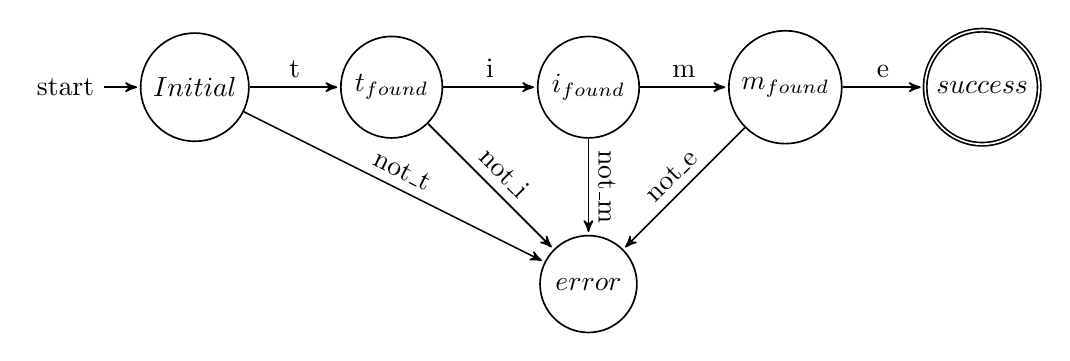
\begin{tikzpicture}[->,>=stealth',shorten >=1pt,auto,node distance=2.5cm, semithick]
		\tikzstyle{every state}=[draw,minimum size=3.5em]
		
		\node[initial,state]       (S1)                       {$Initial$};
		\node[state]       (S2)    [right of=S1]      {$t_{found}$};
		\node[state]       (S3)    [right of=S2]      {$i_{found}$};
		\node[state]       (S4)    [right of=S3]      {$m_{found}$};
		\node[state,accepting]       (S5)    [right of=S4]      {$success$};
		\node[state]       (S6)    [below of=S3]      {$error$};
		
		
		\path 	(S1)   edge          		node[anchor=south, above] {t}     (S2)
		(S2)   edge                 node[anchor=south, above] {i}	  (S3)
		(S3)   edge                 node[anchor=south, above] {m} 	  (S4)
		(S4)   edge   				node[anchor=south, above] {e}     (S5)   
		(S1)   edge          		node[sloped, above] {not\_t}     (S6)
		(S2)   edge                 node[sloped, above] {not\_i}	  (S6)
		(S3)   edge                 node[sloped, above] {not\_m} 	  (S6)
		(S4)   edge   				node[sloped, above] {not\_e}     (S6)   
		;
		\end{tikzpicture}
		\end{adjustbox}
		\caption{Simple FSM parsing the string ``time"}
		\label{fig:FSM}		
	\end{figure}
\end{frame}

\begin{frame}{Timed Automata}
	\begin{itemize}
		\item A timed automaton \cite{Alur:1994:TTA:180782.180519} is a finite state automaton extended with a finite set of real-valued clocks. 
		\item Upon an input, the selection of next state is based not only on the input symbol but also on the time of the current symbol with respect to the formerly read symbols. 
	\end{itemize}
	
	\textbf{Example:} Consider a simple timed automaton in Figure \ref{fig:fig1}. This automaton accepts an input sequence `a' followed by `b' such that, there is 2 units of time difference between any two consecutive a's and b's.
	 
	 \begin{figure}
	 	\centering
	 	\includegraphics[width=0.5\linewidth]{"fig1"}
	 	\caption{A simple timed automaton}
	 	\label{fig:fig1}
	 \end{figure}
\end{frame}

\section{Synthesis of Timed Automata from Scenarios}

\begin{frame}{Synthesis of Timed Automata from Scenarios}
Our method of synthesizing a timed automaton model of a real-time system from scenarios involves two steps:
	\begin{enumerate}
		\item Constructing a time annotated graph from scenarios, and
		\item Constructing a timed automaton from time annotated graph.
	\end{enumerate}
\end{frame}

\begin{frame}{Synthesis of Timed Automata from Scenarios}
	\begin{itemize}
		\item {Our approach for building a formal model is using scenarios. 
			\begin{itemize}
				\item A scenario is a partial description of the behaviour of a system.
				\item A scenario not only describes the events, but also the timing relations among the events.
				\item Set of scenarios together can capture the behaviour of the real-time system.
			\end{itemize}
			}
		\item We use Timed Event Sequences to describe the scenarios formally.
		\item We use Mode graphs to specify the legal events that can occur in the system.
	\end{itemize}	
\end{frame}


\begin{frame}{Mode Graph}
A \emph{mode graph} is a deterministic state machine in which the states are called modes and the transitions triggered by the events in the system. \\
It is a tuple $\mathcal{M} = (M, m_0, m_f, \Sigma, T)$ where,
\begin{itemize}
	\item $M$ is a finite set of modes,
	\item $m_0$ is the initial mode, 
	\item $m_f$ is the final mode, 
	\item $\Sigma$ is a set of events, and 
	\item $T: M\times \Sigma \rightarrow M$ is a
	transition function.
\end{itemize}
\end{frame}

\begin{frame}{Mode Graph Example}
\begin{figure}
	\begin{adjustbox}{max totalsize={.99\textwidth}{.85\textheight},center}
		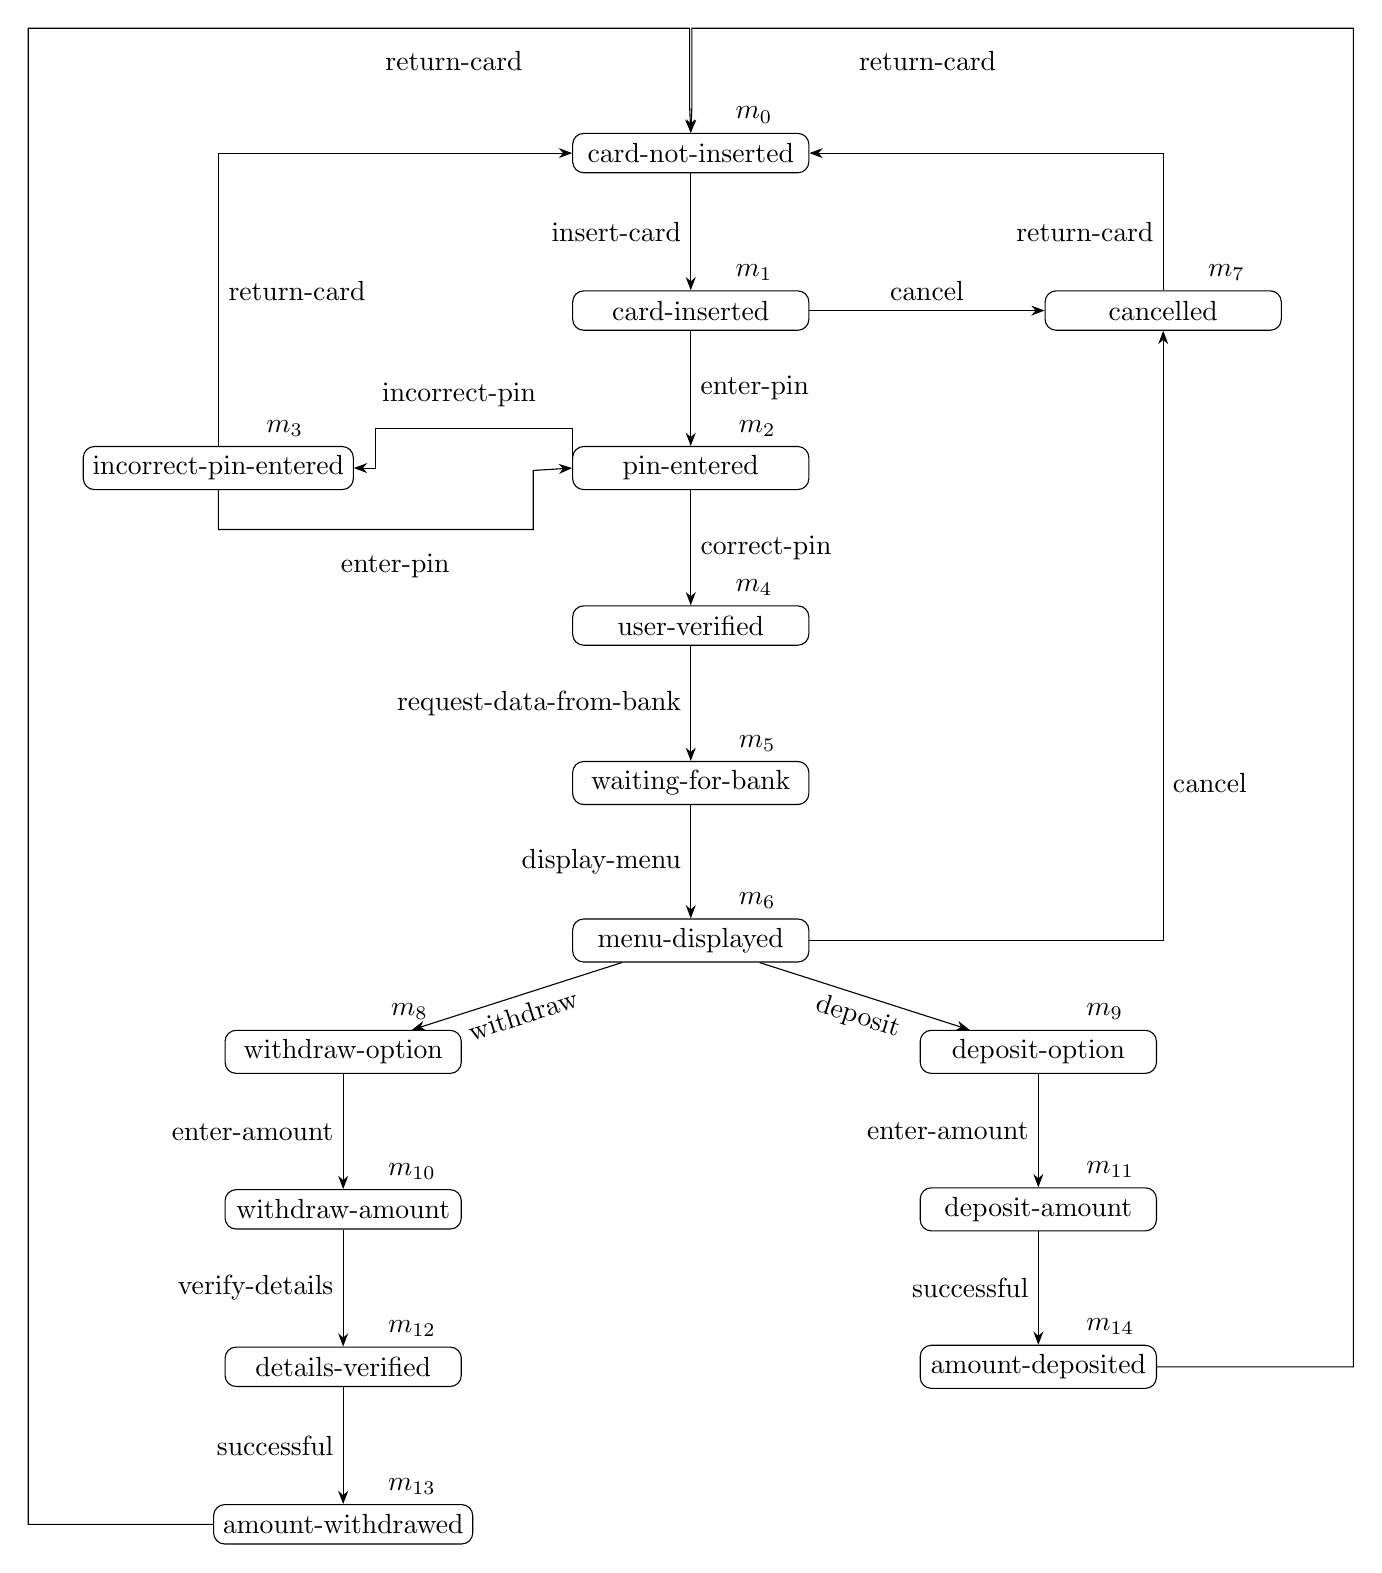
\begin{tikzpicture}[
		node distance=2cm,
		state/.style={rectangle, rounded corners, minimum width=3cm, minimum height=0.5cm,text centered, draw=black},
		process/.style={rectangle, minimum width=3cm, minimum height=0.5cm, text centered, draw=black, fill=orange!30},
		io/.style={trapezium, trapezium left angle=70, trapezium right angle=110, minimum width=3cm, minimum height=1cm, text centered, draw=black, fill=blue!30},
		decision/.style={diamond, minimum width=3cm, minimum height=1cm, text centered, draw=black, fill=green!30},
		]
		
		\node[state]       (m_0) [label={[label]30:$m_0$}]                                        {card-not-inserted};
		\node[state]         (m_1) [below of=m_0, label={[label]30:$m_1$}]                          {card-inserted};
		\node[state]         (m_2) [below of=m_1, label={[label]30:$m_2$}]                          {pin-entered};
		\node[state]         (m_3) [left of=m_2, xshift=-4cm, label={[label]30:$m_3$}]              {incorrect-pin-entered};
		\node[state]         (m_4) [below of=m_2, label={[label]30:$m_4$}]                          {user-verified};
		\node[state]         (m_5) [below of=m_4, label={[label]30:$m_5$}]                          {waiting-for-bank};
		\node[state]         (m_6) [below of=m_5, label={[label]30:$m_6$}]                          {menu-displayed};
		\node[state]         (m_7) [right of=m_1, xshift=4cm, label={[label]30:$m_7$}]              {cancelled};
		\node[state]         (m_8) [below left of=m_6, xshift=-3cm, label={[label]30:$m_8$}]        {withdraw-option};
		\node[state]         (m_9) [below right of=m_6, xshift=3cm, label={[label]30:$m_9$}]        {deposit-option};
		\node[state]         (m_10) [below of=m_8, label={[label]30:$m_{10}$}]                      {withdraw-amount};
		\node[state]         (m_11) [below of=m_9, label={[label]30:$m_{11}$}]                      {deposit-amount};
		\node[state]         (m_12) [below of=m_10, label={[label]30:$m_{12}$}]                     {details-verified};
		\node[state]         (m_13) [below of=m_12, label={[label]30:$m_{13}$}]                     {amount-withdrawed};
		\node[state]         (m_14) [below of=m_11, label={[label]30:$m_{14}$}]                     {amount-deposited};
		
		
		\draw [arrows=-Stealth] (m_0)                                                    --node[anchor=east]                                              {insert-card}        (m_1);
		\draw [arrows=-Stealth] (m_1)                                                    --node[anchor=west]                                              {enter-pin}         (m_2);
		\draw [arrows=-Stealth] (m_1)                                                    --node[anchor=south]                                             {cancel}       (m_7);
		\draw [arrows=-Stealth] (m_2.west) -- ++(0,0.5)  -- ++(-2.5,0) -- ++(0,-0.5)     --node[xshift=1.2cm,yshift=1.2cm,anchor=north,below]             {incorrect-pin}       (m_3.east);
		\draw [arrows=-Stealth] (m_3.south) -- ++(0,-0.5) -- ++(4,0) -- ++(0,0.75)       --node[xshift=-2cm,yshift=-1.5cm,anchor=south]                   {enter-pin}    (m_2.west);
		\draw [arrows=-Stealth] (m_3)                                                    |-node[xshift=1cm,yshift=-1.5cm,anchor=north,below]              {return-card} (m_0);
		\draw [arrows=-Stealth] (m_2)                                                    --node[anchor=west]                                              {correct-pin}       (m_4);
		\draw [arrows=-Stealth] (m_4)                                                    --node[anchor=east]                                              {request-data-from-bank}(m_5);
		\draw [arrows=-Stealth] (m_5)                                                    --node[anchor=east]                                              {display-menu}         (m_6);
		\draw [arrows=-Stealth] (m_6)                                                    -|node[yshift=2cm,anchor=west]                                              {cancel}       (m_7);
		\draw [arrows=-Stealth] (m_7)                                                    |-node[yshift=-1cm,anchor=east]                                              {return-card}    (m_0);
		\draw [arrows=-Stealth] (m_6)                                                    --node[anchor=north,sloped]                                      {withdraw} (m_8);
		\draw [arrows=-Stealth] (m_6)                                                    --node[anchor=north,sloped]                                      {deposit}       (m_9);
		\draw [arrows=-Stealth] (m_8)                                                    --node[anchor=east]                                              {enter-amount}        (m_10);
		\draw [arrows=-Stealth] (m_10)                                                   --node[anchor=east]                                              {verify-details}   (m_12);
		\draw [arrows=-Stealth] (m_12)                                                   --node[anchor=east]                                              {successful}       (m_13);
		\draw [arrows=-Stealth] (m_13) -- ++(-4,0) -- ++(0,19) -- ++(8.4,0) -- ++(0,-1)              --node[xshift=-3cm,yshift=0.5cm,anchor=south]                     {return-card}    (m_0.north);
		\draw [arrows=-Stealth] (m_9)                                                    --node[anchor=east]                                              {enter-amount} (m_11);
		\draw [arrows=-Stealth] (m_11)                                                   --node[anchor=east]                                              {successful}       (m_14);
		\draw [arrows=-Stealth] (m_14) -- ++(4,0) -- ++(0,17) -- ++(-8.4,0) -- ++(0,-1)               -- node[xshift=3cm,yshift=0.5cm,anchor=south]                                            {return-card} (m_0.north);
		
		\end{tikzpicture}
	\end{adjustbox}
	\caption{Mode graph of the ATM}
	\label{fig:Mode graph of the ATM}
\end{figure}
\end{frame}

\begin{frame}{Timed Event Sequences}
	The scenarios describing the partial behaviours of a real-time system are expressed formally in the form of Timed Event Sequences (TES).\\ A Timed Event Sequence $\xi$ contains:
	\begin{columns}
		\begin{column}{0.6\textwidth}
			\begin{enumerate}
				\item The initial mode of the scenario,
				\item The final mode of the scenario,
				\item A set of events and their corresponding time annotations.
			\end{enumerate}
		\end{column}
		\begin{column}{0.4\textwidth}
			\begin{adjustbox}{max totalsize={.99\textwidth}{.80\textheight},center}
			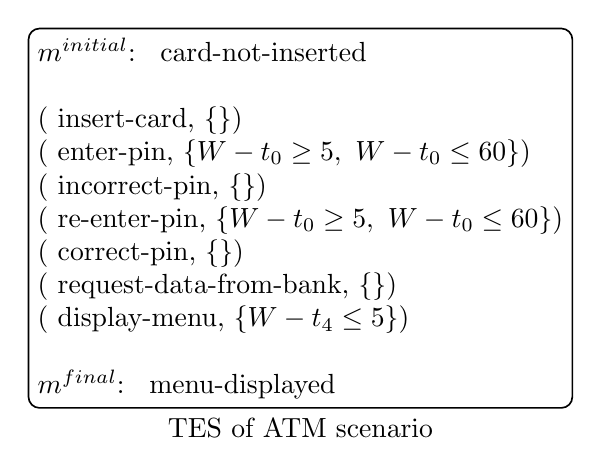
\begin{tikzpicture}[->,>=stealth']
			\tikzset{vertex/.style = {shape=rectangle,rounded corners, semithick, draw,align=left}}
			
			\node[vertex, label = below: TES of ATM scenario] (QUERY) 
			{ $m^{initial}$: { card-not-inserted} \\
				\\
				({ insert-card}, $\{\}$) \\
				({ enter-pin}, $\{W-t_0\geq 5,~W-t_0\leq 60\}$) \\
				({ incorrect-pin}, $\{\}$) \\
				({ re-enter-pin}, $\{W-t_0\geq 5,~W-t_0\leq 60\}$) \\
				({ correct-pin}, $\{\}$) \\
				({ request-data-from-bank}, $\{\}$) \\
				({ display-menu}, $\{W-t_4\leq 5\}$) \\
				\\
				$m^{final}$: { menu-displayed}
			};
			
			\end{tikzpicture}
			\end{adjustbox}
		\end{column}
	\end{columns}
	
\end{frame}

\begin{frame}{Dominance Assumption}
	\begin{itemize}
		\item Given two modes $m_i$ and $m_j$, $m_i$ is said to be the \emph{dominating mode} of $m_j$ iff all the paths to $m_j$ from the initial mode in the mode graph pass through $m_i$ \cite{Lengauer:1979}. We call this the \emph{Dominance} relation and denote it as \emph{$m_i$ DOM $m_j$}.
		\item Dominance assumption ensures that time variables are well defined.
	\end{itemize}
\end{frame}


\begin{frame}{Dominance Assumption Example}
	\begin{figure}[!h]
	%	\begin{minipage}[b]{.3\textwidth}
			\begin{adjustbox}{max totalsize={.80\textwidth}{.50\textheight},center}
			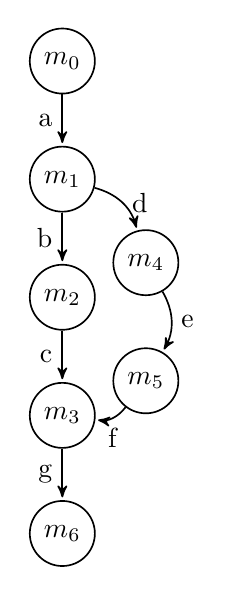
\begin{tikzpicture}[->,>=stealth',shorten >=1pt,auto,node distance=1.5cm,
			semithick]
			\tikzstyle{every state}=[draw,minimum size=1em]
			
			\node[state]       (S_0)                    {$m_0$};
			\node[state]         (S_1) [below of=S_0]     {$m_1$};
			\node[state]         (S_2) [below of=S_1]     {$m_2$};
			\node[state]         (S_3) [below of=S_2]     {$m_3$};
			\node[state]         (S_4) [below right of=S_1]   {$m_4$};
			\node[state]         (S_5) [below  of=S_4]    {$m_5$};
			\node[state]         (S_6) [below of=S_3]     {$m_6$};
				
			\path (S_0) edge              node[left]  {a}  (S_1)
			(S_1) edge              node[left]  {b}  (S_2)
			(S_2) edge              node[left]  {c}  (S_3)
			(S_1) edge [bend left]  node[right] {d}  (S_4)
			(S_4) edge [bend left]  node[right] {e}  (S_5)
			(S_5) edge [bend left]  node[below] {f}  (S_3)
			(S_3) edge              node[left]  {g}  (S_6)
			
			;
			\end{tikzpicture}
	%	\end{minipage}
		\hspace{1cm}
	%	\begin{minipage}[b]{.3\textwidth}
			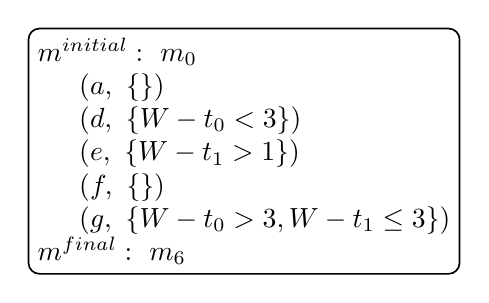
\begin{tikzpicture}[->,>=stealth']
			\tikzset{vertex/.style = {shape=rectangle,rounded corners, semithick, draw,align=left}}
			\node[vertex] (QUERY) 
			{$m^{initial}:~m_0$ \\
				
				\indent    ($a,~\{\}$) \\
				\indent    ($d,~\{W-t_0 < 3\}$) \\
				\indent    ($e,~ \{W-t_1 > 1\}$) \\
				\indent    ($f,~\{\}$) \\
				\indent   ($g,~\{W-t_0 > 3, W-t_1\leq 3\}$) \\
				
				$m^{final}:~m_6$};
			\end{tikzpicture}		
	%	\end{minipage}
		\end{adjustbox}
		\caption{A mode graph and a scenario satisfying the dominance assumption}
		\label{fig:Dominance Assumption}
	\end{figure} 
	\begin{itemize}
		\item $m_0$ and $m_1$ are dominating modes of $m_3$,
		\item Transition $g$ is dominated by all the modes that dominate $m_3$,
		\item $t_0$ and $t_1$, on transition $g$ refer to the modes $m_0$ and $m_1$.
	\end{itemize}
\end{frame}

\begin{frame}{Constructing a Time Annotated Graph from Scenarios}
Given a mode graph $\mathcal{M}$ and a set of Timed Event Sequences  $\Xi = \{\xi_1,\xi_2,..,\xi_k\}$ as inputs, our algorithm synthesizes a time annotated graph (TAG) G \cite{FromScenariosToTimedAutomata-2016}. Initially we start with an empty graph, $G_0$ and perform the following steps:
\begin{enumerate}
	\item Build a partial graph $G_1$ using the first scenario $\xi_1$,
	\item The algorithm repeatedly takes a partially built graph $G_k$, and a scenario $\xi_{k+1} ~(1 < k < n)$ and then generates a new partial graph $G_{k+1}$
\end{enumerate}
Decision on whether to create new states and transitions is resolved with the help of state labels (modes).
A new state $s$ is created and labelled with a mode $m_j$ if there is an event $e$ from state $q$ such that $L(q) = m_i$ and $(m_i,e,m_j) \in T$.
\end{frame}

\begin{frame}{Properties of Constructed Time Annotated Graph}
The graph constructed by algorithm has the following properties:
	\begin{enumerate}
		\item
		It is acyclic,%: as we do not introduce a transition from a state to it's previous states.
		\item
		The graph is connected,%, because the input set of TES is complete.
		\item\label{p3}
		By construction, two states have the same label only if one is a predecessor of the other, %We create a new state with the same label only to avoid introducing a transition from a state to it's predecessor.
		\item\label{p4} The graph is finite,
%		There must be at least one state with no outgoing transitions, because the graph is finite.
		\item
		The graph is deterministic,%: we only add a new transition only if it does not exist from state $s$.
		\item
		The graph is minimal, %because:
%		\begin{itemize}
%			\item
%			We do not add additional states if the state with mode information $m_i$ already exists. We only add in cases when the addition of a new transition creates a cycle.
%			\item
%			In case of multiple existing states, we choose the state that was created first.
%		\end{itemize}
		\item
		After construction, every scenario is a partial run of the constructed graph, and
		\item
		Every path in the final graph is identical to that of the mode graph. %because our algorithm adds a new state or transition based on the mode and transition information in the mode graph.
	\end{enumerate}

\end{frame}


\begin{frame}{Constructing a Timed Automaton from Time Annotated Graph}
	To convert a time annotated graph to a timed automaton we have to:
	\begin{enumerate}	
		\item Determine the required number of clocks,
		\item Add clock resets, and
		\item Replace the time annotations with the clock constraints
	\end{enumerate}
	\underline{Example}: If there is a time annotation $W-t_0 > 5$ on a transition, then the clock constraint $c_0 > 5$ is added to that transition and clock $c_0$ is reset on all transitions from the state labelled with mode $m_0$.
\end{frame}

\begin{frame}{Example}
	\begin{figure}
		\begin{adjustbox}{max totalsize={.99\textwidth}{.85\textheight},center}
		%	\begin{minipage}{.7\textwidth}
		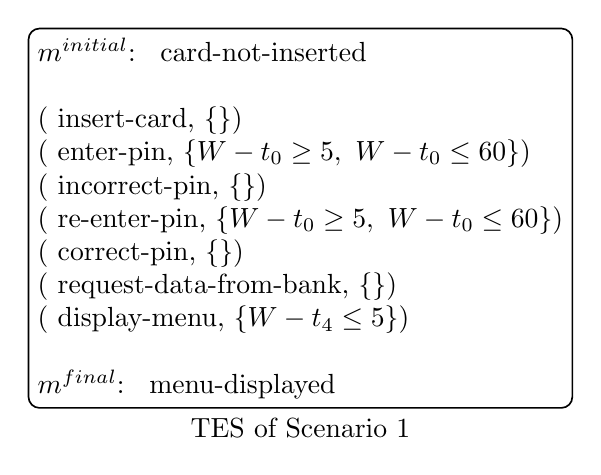
\begin{tikzpicture}[->,>=stealth']
		\tikzset{vertex/.style = {shape=rectangle,rounded corners, semithick, draw,align=left}}
		
		\node[vertex, label = below: TES of Scenario 1] (QUERY) 
		{ $m^{initial}$: { card-not-inserted} \\
			\\
			({ insert-card}, $\{\}$) \\
			({ enter-pin}, $\{W-t_0\geq 5,~W-t_0\leq 60\}$) \\
			({ incorrect-pin}, $\{\}$) \\
			({ re-enter-pin}, $\{W-t_0\geq 5,~W-t_0\leq 60\}$) \\
			({ correct-pin}, $\{\}$) \\
			({ request-data-from-bank}, $\{\}$) \\
			({ display-menu}, $\{W-t_4\leq 5\}$) \\
			\\
			$m^{final}$: { menu-displayed}
		};
		
		\end{tikzpicture}
		%\end{minipage}
		\hspace{0.5cm}
		%	\begin{minipage}{.7\textwidth}
		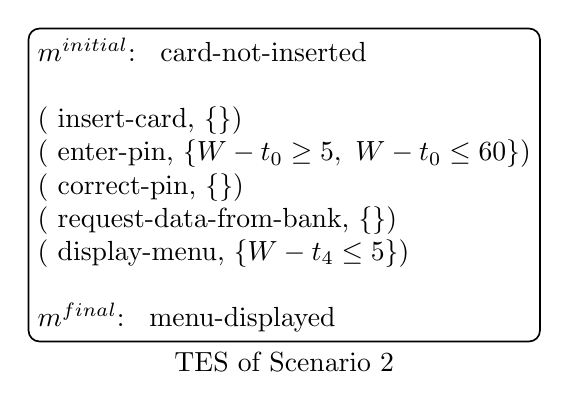
\begin{tikzpicture}[->,>=stealth']
		\tikzset{vertex/.style = {shape=rectangle,rounded corners, semithick, draw,align=left}}
		\node[vertex, label = below: TES of Scenario 2] (QUERY) 
		{ $m^{initial}$: { card-not-inserted} \\
			\\
			({ insert-card}, $\{\}$) \\
			({ enter-pin}, $\{W-t_0\geq 5,~W-t_0\leq 60\}$) \\
			({ correct-pin}, $\{\}$) \\
			({ request-data-from-bank}, $\{\}$) \\
			({ display-menu}, $\{W-t_4\leq 5\}$) \\
			\\
			$m^{final}$: { menu-displayed}
		};
		
		\end{tikzpicture}
		%	\end{minipage}
		\end{adjustbox}
		\caption{Timed Event Sequences of the ATM}
		\label{fig:TES of ATM}
	\end{figure}
\end{frame}

\begin{frame}{Example (Cont.)}

	 \begin{figure}[htp]
	 \centering
	 \includegraphics[width=0.9\columnwidth,height=0.8\textheight]{"ModeGraph"}
	 \caption{Mode Graph for ATM}
	 \label{fig:Mode Graph for ATM}
	 \end{figure}
\end{frame}

\begin{frame}{Example (Cont.)}
	\begin{columns}
		\begin{column}{0.5\textwidth}
			\begin{figure}
				\begin{adjustbox}{max totalsize={.99\textwidth}{.75\textheight},center}
					\begin{tikzpicture}[->,>=stealth',shorten >=1pt,auto,node distance=2.5cm,
					semithick]
					\tikzstyle{every state}=[shape=rectangle,draw]
					
					\node[state]       (S_0)                {$S_0$[$m_0$]};
					\node[state]         (S_1) [below of=S_0] {$S_1$[$m_1$]};
					\node[state]         (S_2) [below of=S_1] {$S_2$[$m_2$]};
					\node[state]         (S_3) [below of=S_2] {$S_3$[$m_3$]};
					\node[state]         (S_4) [below of=S_3] {$S_4$[$m_2$]};
					\node[state]         (S_5) [below of=S_4] {$S_5$[$m_4$]};
					\node[state]         (S_6) [below of=S_5] {$S_6$[$m_5$]};
					\node[state]         (S_7) [below of=S_6] {$S_7$[$m_6$]};
					
					
					\path (S_0) edge              node[left] {insert-card}                (S_1)
					(S_1) edge              node[left] {enter-pin [$W − t_0 \ge 5, W − t_0 \le 60$]}  (S_2)
					(S_2) edge        node[left] {incorrect-pin}              (S_3)
					(S_3) edge              node[left] {enter-pin [$W − t_0 \ge 5, W − t_0 \le 60$]}  (S_4)
					(S_4) edge              node[left] {correct-pin} (S_5)
					(S_5) edge        node[left] {request-data-from-bank} (S_6)
					(S_6) edge        node[left] {display-menu [$W − t_4 \le 5$]} (S_7)
					(S_2) edge [bend left]  node[right] {correct-pin} (S_5)
					;
					\end{tikzpicture}
			
				\end{adjustbox}
				\caption{Time annotated graph synthesized from two TES in Figure \ref{fig:TES of ATM}}
				\label{fig:Time annotated graph generated by combining scenario 1 and scenario 2}
			\end{figure}			
		\end{column}
	
		\begin{column}{0.5\textwidth}
			\begin{figure}[!htb]
				\begin{adjustbox}{max totalsize={.99\textwidth}{.8\textheight},center}
					\begin{tikzpicture}[->,>=stealth',shorten >=1pt,auto,node distance=2.5cm,
					semithick]
					\tikzstyle{every state}=[draw]
					
					\node[state]       (S_0)                {$S_0$};
					\node[state]         (S_1) [below of=S_0] {$S_1$};
					\node[state]         (S_2) [below of=S_1] {$S_2$};
					\node[state]         (S_3) [below of=S_2] {$S_3$};
					\node[state]         (S_4) [below of=S_3] {$S_4$};
					\node[state]         (S_5) [below of=S_4] {$S_5$};
					\node[state]         (S_6) [below of=S_5] {$S_6$};
					\node[state]         (S_7) [below of=S_6] {$S_7$};
					
					
					\path (S_0) edge              node[left] {insert-card [$c_0 :=0$]}                (S_1)
					(S_1) edge              node[left] {enter-pin [$c_0 \ge 5, c_0 \le 60$]}  (S_2)
					(S_2) edge        node[left] {incorrect-pin}              (S_3)
					(S_3) edge              node[left] {enter-pin [$c_0 \ge 5, c_0 \le 60$]}  (S_4)
					(S_4) edge              node[left] {correct-pin} (S_5)
					(S_5) edge        node[left] {request-data-from-bank [$c_4 :=0$]} (S_6)
					(S_6) edge        node[left] {display-menu [$c_4 \le 5$]} (S_7)
					(S_2) edge [bend left]  node[right] {correct-pin} (S_5)
					;
					\end{tikzpicture}
				\end{adjustbox}
				\caption{Timed automaton constructed from time annotated graph in Figure \ref{fig:Time annotated graph generated by combining scenario 1 and scenario 2}}
				\label{fig:Timed Automaton generated by combining scenario 1 and scenario 2}
			\end{figure}	
			
		\end{column}
	\end{columns}

\end{frame}

\section{Optimal Clock Allocation of Timed Automata}

\begin{frame}{Class of Timed Automata}
The timed automaton constructed as a result of our synthesis method belongs to the class of timed automata that satisfies these properties:
	\begin{enumerate}
		\item{The automaton is connected and has a unique initial state $s_0$,}%Every state is reachable from $s_0$},
		\item{A clock constraint on a transition `$r$' can only refer to the times of transitions from states that dominate the transition `$r$', we call this \textit{dominance assumption}},
		\item{A clock $t_j$ can only be reset on a transition leaving a state $s$, where label is $j$, that is $L(s)=j$.}
	\end{enumerate}
\end{frame}

\begin{frame}{Optimal Clock Allocation of Timed Automata}

Given a timed automaton $\cal A$ that belongs to the aforementioned class of timed automata, to transform it to an equivalent timed automaton $\cal A'$ with optimal allocation of clocks, we need to perform the following steps in order:
\begin{enumerate}
	\item{Calculate the liveness ranges of clocks in the timed automaton $\cal A$,}
	\item{Replace the original clocks in $\cal A$ with a set of new clocks,} %such that $|P|\le|V|$,}
	%\item{Replace the original clocks in $A ~(V=\left\{t_0,t_1,...,t_n \right\}$) with a set of new clocks $P=\left \{c_0,c_1,..,c_m \right\}$ such that $|P|\le|V|$}
	\item{Rewrite the clock constraints and clock resets in $\cal A$ in terms of new clock variables.}
\end{enumerate}
%\begin{itemize}
%	\item Liveness analysis
%	\item Clock allocation
%\end{itemize}
\end{frame}

\begin{frame}{Liveness Range Analysis}
Liveness Ranges of all the clocks in a timed automaton helps us determine if a particular clock is only on these transitions.
\begin{itemize}
	\item Let $\cal A$ $= (E, Q, \{q^0\}, Q_f, V, R, L)$ be the timed automaton and $r = (s, s', e, \lambda_r, \phi_r) \in R$ be a transition.
	\item Let $N = \{j~|~t_j\sim a \in \phi \vee t_j \in \lambda$, where $(s, s', e, \lambda_r, \phi_r) \in R\}$, be a set of \emph{clock numbers} used to denote subscripts of the clocks on all the transitions in $R$.
\end{itemize}
\end{frame}

\begin{frame}{Liveness Range Analysis}
	The following are a set of functions used to calculate the liveness ranges:
	\begin{itemize}
		\item
		$\mathit{\textbf{clock\_ref}}$: $\mathit{clock\_ref(r)}$ is the set of clocks which are referred to in the clock constraints on $r$.
		
		\item
		$\textbf{born}$: $\Born(r)$ identifies a clock that is reset on $r$  whose value can be used on some transition	reachable from $r$.
	
		\item 
		$\textbf{active}$: $\Active(r)$ identifies clocks that are ``alive'' on $r$ (i.e., their  values may be subsequently used). Notice that $\Born(r)\subseteq \Active(r)$.
		
		\item
		$\textbf{needed}$: Maps transition $r$ to $\Active(r)\cup \mathit{clock\_ref(r)}$.
		
	\end{itemize}

\end{frame}

\begin{frame}{Liveness Range Analysis Example}
 \begin{columns}
	\begin{column}{0.4\textwidth}
		\begin{figure}
			\begin{adjustbox}{max totalsize={.99\textwidth}{.8\textheight},center}
			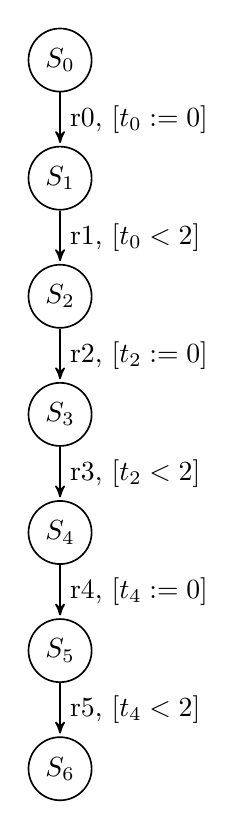
\begin{tikzpicture}[->,>=stealth',shorten >=1pt,auto,node distance=1.5cm,
			semithick]
			\tikzstyle{every state}=[draw,minimum size=1em]
			
			\node[state]         (S_0)                    {$S_0$};
			\node[state]         (S_1) [below of=S_0]     {$S_1$};
			\node[state]         (S_2) [below of=S_1]     {$S_2$};
			\node[state]         (S_3) [below of=S_2]     {$S_3$};
			\node[state]         (S_4) [below of=S_3]     {$S_4$};
			\node[state]         (S_5) [below of=S_4]     {$S_5$};
			\node[state]         (S_6) [below of=S_5]     {$S_6$};	
			
			\path (S_0) edge              node[right]  {r0, [$t_0:=0$]}  (S_1)
			(S_1) edge              node[right]  {r1, [$t_0<2$]}   (S_2)
			(S_2) edge              node[right]  {r2, [$t_2:=0$]}  (S_3)
			(S_3) edge              node[right] {r3, [$t_2<2$]}   (S_4)
			(S_4) edge              node[right] {r4, [$t_4:=0$]}  (S_5)
			(S_5) edge              node[right] {r5, [$t_4<2$]}   (S_6)
			
			;
			\end{tikzpicture}
			\end{adjustbox}
			\caption{A simple timed automaton}
			\label{fig:Simple Timed Automaton}
		\end{figure}
	\end{column}
			\begin{column}{0.5\textwidth}
			\begin{table}
				\centering
				\caption{$born$ and $active$ values}
				\label{tab:table1}
				\begin{tabular}{ccc}
					\toprule
					{ \textbf{Transition}} & { \textbf{Born}} & { \textbf{Active}} \\ \midrule
					{ $r_0$}               & { \{0\}}         & { \{0\}}           \\
					{ $r_1$}               & { $\phi$}        & { $\phi$}          \\
					{ $r_2$}               & { \{2\}}         & { \{2\}}           \\
					{ $r_3$}               & { $\phi$}        & { $\phi$}          \\
					{ $r_4$}               & { \{4\}}         & { \{4\}}           \\
					{ $r_5$}               & { $\phi$}        & { $\phi$} \\
					\bottomrule
				\end{tabular}
			\end{table}
		\end{column}
		\begin{column}{0.1\textwidth}
		\end{column}
	\end{columns}
\end{frame}

\begin{frame}{Clock Allocation}
	The liveness analysis algorithm calculates liveness ranges and generates extended transitions of the form $(r,born(r),active(r))$. Our method to optimally allocate the clocks revolves around the idea that: 
	\begin{itemize}
		\item A clock can be reused if the active range of the clock has ended,
		\item The clock cannot be reused on a transition if the transition belongs to active range of that clock.
	\end{itemize}

\end{frame}

\begin{frame}{Clock Allocation}
	\begin{definition}
		Given a timed automaton $\cal A$ with the set $R$ of (extended) transitions and the set $N$ of clock numbers, a \emph{clock allocation} for $\cal A$ is a relation $\Var{alloc}\subset R\times P_0\times N$ such that $(r, c, j)\in \Var{alloc} \Rightarrow j\in \Var{active(r)}$.
	\end{definition}
	\begin{columns}
		\begin{column}{0.4\textwidth}
			\begin{figure}
				\begin{adjustbox}{max totalsize={.80\textwidth}{.55\textheight},center}
				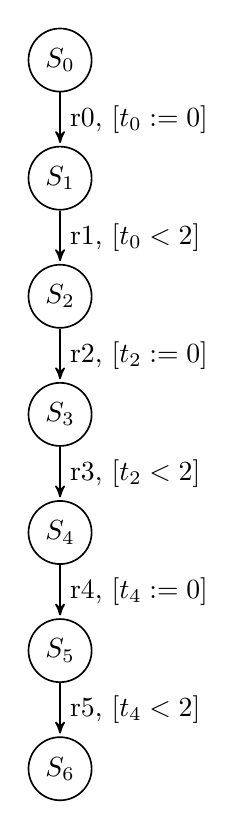
\begin{tikzpicture}[->,>=stealth',shorten >=1pt,auto,node distance=1.5cm,
				semithick]
				\tikzstyle{every state}=[draw,minimum size=1em]
				
				\node[state]         (S_0)                    {$S_0$};
				\node[state]         (S_1) [below of=S_0]     {$S_1$};
				\node[state]         (S_2) [below of=S_1]     {$S_2$};
				\node[state]         (S_3) [below of=S_2]     {$S_3$};
				\node[state]         (S_4) [below of=S_3]     {$S_4$};
				\node[state]         (S_5) [below of=S_4]     {$S_5$};
				\node[state]         (S_6) [below of=S_5]     {$S_6$};	
				
				\path (S_0) edge              node[right]  {r0, [$t_0:=0$]}  (S_1)
				(S_1) edge              node[right]  {r1, [$t_0<2$]}   (S_2)
				(S_2) edge              node[right]  {r2, [$t_2:=0$]}  (S_3)
				(S_3) edge              node[right] {r3, [$t_2<2$]}   (S_4)
				(S_4) edge              node[right] {r4, [$t_4:=0$]}  (S_5)
				(S_5) edge              node[right] {r5, [$t_4<2$]}   (S_6)
				
				;
				\end{tikzpicture}
				\end{adjustbox}
				\caption{A simple timed automaton}
		
			\end{figure}
		\end{column}
		\begin{column}{0.5\textwidth}
			$\Var{alloc}~$=$\{(r_0,c_0,0), (r_1,c_0,0), (r_2,c_0,0), $\\ $(r_3,c_0,0),(r_4,c_0,0), (r_5,c_0,0), (r_6,c_0,0), $\\$(r_1,c_1,1),(r_2,c_1,1), (r_3,c_1,1), (r_4,c_1,1)\} $
		\end{column}
		\begin{column}{0.1\textwidth}
			
		\end{column}
	\end{columns}

\end{frame}

\begin{frame}{Problematic states}

	\begin{figure}
		\begin{adjustbox}{max totalsize={.90\textwidth}{.45\textheight},center}
		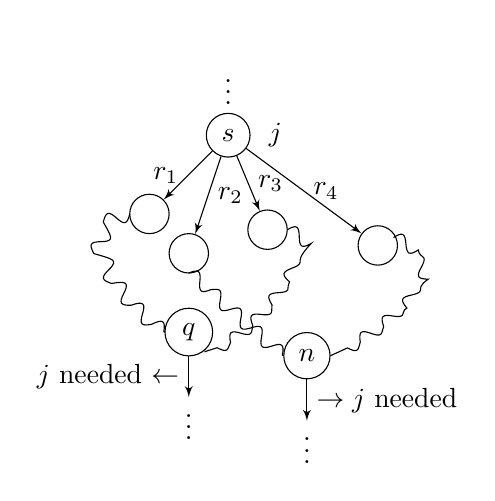
\begin{tikzpicture}
		
		\tikzset{vertex/.style = {shape=circle,draw,minimum size=0.5cm}}
		\tikzset{vertex2/.style = {shape=circle,draw=none,minimum size=0.5cm}}
		\tikzset{edge/.style = {->,> = latex'}}
		% vertices
		\node[vertex] (a) at  (0,0) {$s$};
		\node[vertex] (b) at  (-1,-1) {};
		\node[vertex] (c) at  (-0.5,-1.5) {};
		\node[vertex] (d) at  (0.5,-1.2) {};
		\node[vertex] (e) at  (1.9,-1.4) {};
		
		\node[vertex] (f) at  (-0.5,-2.5) {$q$};
		\node[vertex] (g) at  (1,-2.8) {$n$};
		
		\node[vertex2] (bm) at  (0.6,0) {$j$};
		%\node[vertex2] (label) at  (0,-4.7) {(b)};
		
		\node [shape=circle,minimum size=0.5em] (a1) at (0,1.2) {};
		
		\node [shape=circle,minimum size=0.5em] (c1) at (-0.5,-3.5) {};
		\node [shape=circle,minimum size=0.5em] (c2) at (-0.5,-3.7) {};
		
		\node [shape=circle,minimum size=0.5em] (d1) at (1,-3.8) {};
		\node [shape=circle,minimum size=0.5em] (d2) at (1,-4) {};
		
		\draw[edge] (f) to node[left]{$j$ needed $\leftarrow $} (c1) ;
		\draw[edge] (g) to node[right]{$\rightarrow j$ needed} (d1) ;
		
		\path (c1) to node {\vdots} (c2);
		\path (d1) to node {\vdots} (d2);
		
		%edges
		\draw[edge] (a) to node[left]{$r_1$} (b) ;
		\draw[edge] (a) to node[right]{$r_2$} (c) ;
		\draw[edge] (a) to node[right]{$r_3$} (d) ;
		\draw[edge] (a) to node[right]{$r_4$} (e) ;
		
		\path (a1) to node {\vdots} (a);
		
		\draw [decorate, decoration={coil,aspect=0}]
		{ (-1.25,-1) .. controls (-1.9,-1.2) and (-1.5,-2) .. (-0.8,-2.5) };
		
		\draw [decorate, decoration={coil,aspect=0}]
		{ (0.75,-1.2) .. controls (1.1,-1.4) and (0.5,-2.5) .. (-0.3,-2.75) };
		
		\draw [decorate, decoration={coil,aspect=0}]
		{ (-0.5,-1.75) .. controls (-0.3,-1.9) and (0,-2.2) .. (0.7,-2.8) };
		
		\draw [decorate, decoration={coil,aspect=0}]
		{ (2.1,-1.3) .. controls (2.9,-1.7) and (2,-2.5) .. (1.3,-2.8) };
		
		\end{tikzpicture}
		\end{adjustbox}
		\caption{A timed automaton with problematic states}
		\label{twofamilies}		
	\end{figure}
%	Consider example shown in Figure \ref{twofamilies}:
	\begin{itemize}
		\item Clock $t_j$ is born on all outgoing transition of state $s$.
		\item $r_1$, $r_3$ meet at state $q$ and $r_2$, $r_4$ meet at state $n$.
	\end{itemize}
	States $q$ and $n$ are the \emph{problematic} states. So, $r_1,r_3$ should be assigned the same clock and $r_2,r_4$ should be assigned the same clock.
\end{frame}

\begin{frame}{Mode Graph}
	\begin{figure}
		\begin{adjustbox}{max totalsize={.99\textwidth}{.85\textheight},center}
			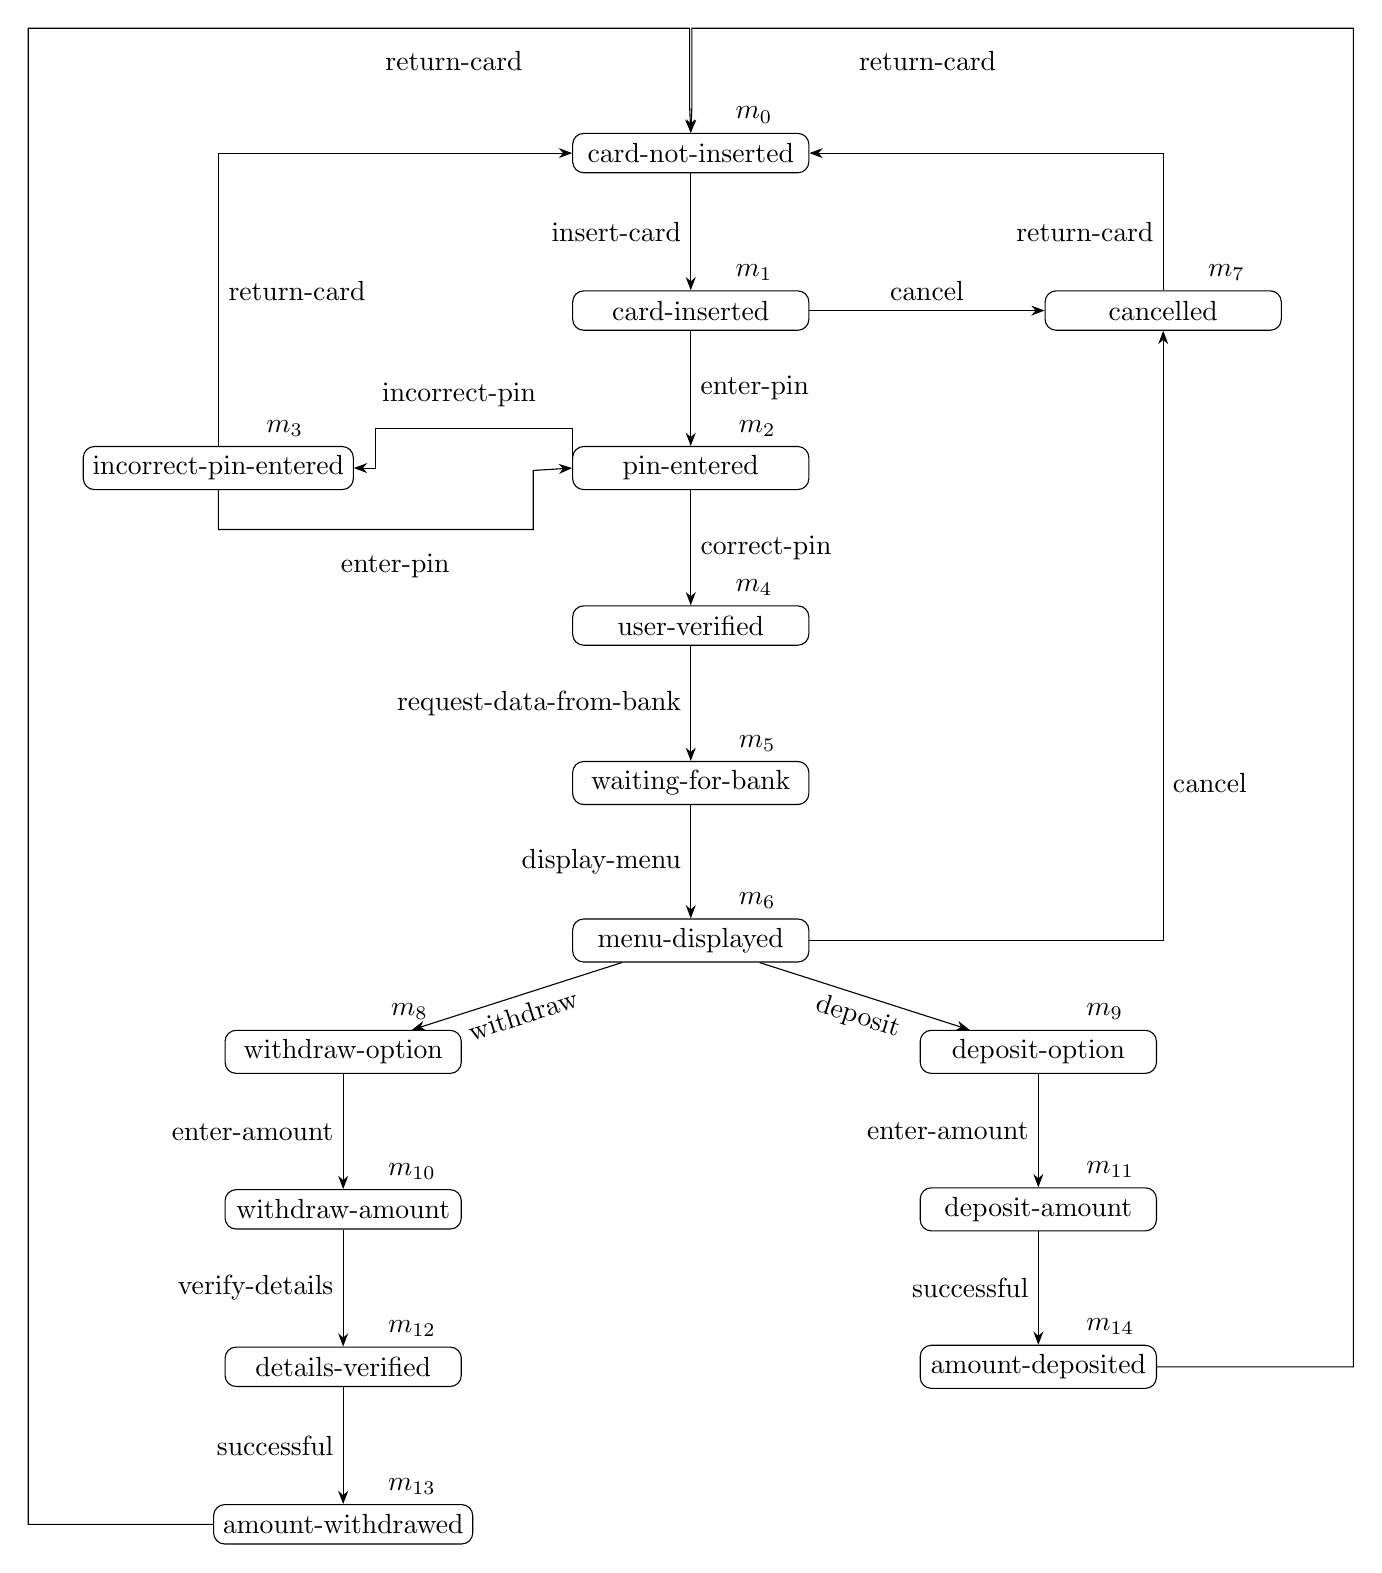
\begin{tikzpicture}[
			node distance=2cm,
			state/.style={rectangle, rounded corners, minimum width=3cm, minimum height=0.5cm,text centered, draw=black},
			process/.style={rectangle, minimum width=3cm, minimum height=0.5cm, text centered, draw=black, fill=orange!30},
			io/.style={trapezium, trapezium left angle=70, trapezium right angle=110, minimum width=3cm, minimum height=1cm, text centered, draw=black, fill=blue!30},
			decision/.style={diamond, minimum width=3cm, minimum height=1cm, text centered, draw=black, fill=green!30},
			]
			
			\node[state]       (m_0) [label={[label]30:$m_0$}]                                        {card-not-inserted};
			\node[state]         (m_1) [below of=m_0, label={[label]30:$m_1$}]                          {card-inserted};
			\node[state]         (m_2) [below of=m_1, label={[label]30:$m_2$}]                          {pin-entered};
			\node[state]         (m_3) [left of=m_2, xshift=-4cm, label={[label]30:$m_3$}]              {incorrect-pin-entered};
			\node[state]         (m_4) [below of=m_2, label={[label]30:$m_4$}]                          {user-verified};
			\node[state]         (m_5) [below of=m_4, label={[label]30:$m_5$}]                          {waiting-for-bank};
			\node[state]         (m_6) [below of=m_5, label={[label]30:$m_6$}]                          {menu-displayed};
			\node[state]         (m_7) [right of=m_1, xshift=4cm, label={[label]30:$m_7$}]              {cancelled};
			\node[state]         (m_8) [below left of=m_6, xshift=-3cm, label={[label]30:$m_8$}]        {withdraw-option};
			\node[state]         (m_9) [below right of=m_6, xshift=3cm, label={[label]30:$m_9$}]        {deposit-option};
			\node[state]         (m_10) [below of=m_8, label={[label]30:$m_{10}$}]                      {withdraw-amount};
			\node[state]         (m_11) [below of=m_9, label={[label]30:$m_{11}$}]                      {deposit-amount};
			\node[state]         (m_12) [below of=m_10, label={[label]30:$m_{12}$}]                     {details-verified};
			\node[state]         (m_13) [below of=m_12, label={[label]30:$m_{13}$}]                     {amount-withdrawed};
			\node[state]         (m_14) [below of=m_11, label={[label]30:$m_{14}$}]                     {amount-deposited};
			
			
			\draw [arrows=-Stealth] (m_0)                                                    --node[anchor=east]                                              {insert-card}        (m_1);
			\draw [arrows=-Stealth] (m_1)                                                    --node[anchor=west]                                              {enter-pin}         (m_2);
			\draw [arrows=-Stealth] (m_1)                                                    --node[anchor=south]                                             {cancel}       (m_7);
			\draw [arrows=-Stealth] (m_2.west) -- ++(0,0.5)  -- ++(-2.5,0) -- ++(0,-0.5)     --node[xshift=1.2cm,yshift=1.2cm,anchor=north,below]             {incorrect-pin}       (m_3.east);
			\draw [arrows=-Stealth] (m_3.south) -- ++(0,-0.5) -- ++(4,0) -- ++(0,0.75)       --node[xshift=-2cm,yshift=-1.5cm,anchor=south]                   {enter-pin}    (m_2.west);
			\draw [arrows=-Stealth] (m_3)                                                    |-node[xshift=1cm,yshift=-1.5cm,anchor=north,below]              {return-card} (m_0);
			\draw [arrows=-Stealth] (m_2)                                                    --node[anchor=west]                                              {correct-pin}       (m_4);
			\draw [arrows=-Stealth] (m_4)                                                    --node[anchor=east]                                              {request-data-from-bank}(m_5);
			\draw [arrows=-Stealth] (m_5)                                                    --node[anchor=east]                                              {display-menu}         (m_6);
			\draw [arrows=-Stealth] (m_6)                                                    -|node[yshift=2cm,anchor=west]                                              {cancel}       (m_7);
			\draw [arrows=-Stealth] (m_7)                                                    |-node[yshift=-1cm,anchor=east]                                              {return-card}    (m_0);
			\draw [arrows=-Stealth] (m_6)                                                    --node[anchor=north,sloped]                                      {withdraw} (m_8);
			\draw [arrows=-Stealth] (m_6)                                                    --node[anchor=north,sloped]                                      {deposit}       (m_9);
			\draw [arrows=-Stealth] (m_8)                                                    --node[anchor=east]                                              {enter-amount}        (m_10);
			\draw [arrows=-Stealth] (m_10)                                                   --node[anchor=east]                                              {verify-details}   (m_12);
			\draw [arrows=-Stealth] (m_12)                                                   --node[anchor=east]                                              {successful}       (m_13);
			\draw [arrows=-Stealth] (m_13) -- ++(-4,0) -- ++(0,19) -- ++(8.4,0) -- ++(0,-1)              --node[xshift=-3cm,yshift=0.5cm,anchor=south]                     {return-card}    (m_0.north);
			\draw [arrows=-Stealth] (m_9)                                                    --node[anchor=east]                                              {enter-amount} (m_11);
			\draw [arrows=-Stealth] (m_11)                                                   --node[anchor=east]                                              {successful}       (m_14);
			\draw [arrows=-Stealth] (m_14) -- ++(4,0) -- ++(0,17) -- ++(-8.4,0) -- ++(0,-1)               -- node[xshift=3cm,yshift=0.5cm,anchor=south]                                            {return-card} (m_0.north);
			
			\end{tikzpicture}
		\end{adjustbox}
			\caption{Mode graph of the ATM}
			\label{fig:Mode graph of the ATM}
	\end{figure}
\end{frame}

\section{Case Studies}

\begin{frame}{Automated Teller Machine (ATM)}
Explain original scenario
\end{frame}

\begin{frame}{Automated Teller Machine (ATM)}
	\begin{figure}
		\begin{adjustbox}{max totalsize={.99\textwidth}{.85\textheight},center}
		%	\begin{minipage}{.7\textwidth}
			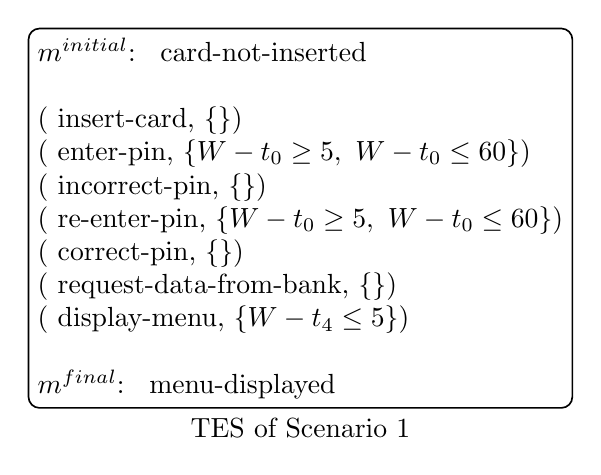
\begin{tikzpicture}[->,>=stealth']
			\tikzset{vertex/.style = {shape=rectangle,rounded corners, semithick, draw,align=left}}
			
			\node[vertex, label = below: TES of Scenario 1] (QUERY) 
			{ $m^{initial}$: { card-not-inserted} \\
				\\
				({ insert-card}, $\{\}$) \\
				({ enter-pin}, $\{W-t_0\geq 5,~W-t_0\leq 60\}$) \\
				({ incorrect-pin}, $\{\}$) \\
				({ re-enter-pin}, $\{W-t_0\geq 5,~W-t_0\leq 60\}$) \\
				({ correct-pin}, $\{\}$) \\
				({ request-data-from-bank}, $\{\}$) \\
				({ display-menu}, $\{W-t_4\leq 5\}$) \\
				\\
				$m^{final}$: { menu-displayed}
			};
			
			\end{tikzpicture}
		%\end{minipage}
		\hspace{0.5cm}
	%	\begin{minipage}{.7\textwidth}
			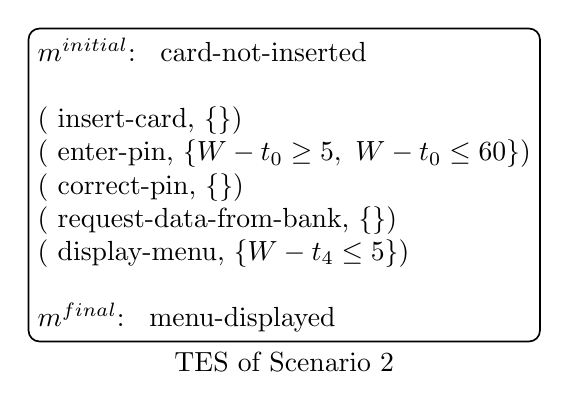
\begin{tikzpicture}[->,>=stealth']
			\tikzset{vertex/.style = {shape=rectangle,rounded corners, semithick, draw,align=left}}
			\node[vertex, label = below: TES of Scenario 2] (QUERY) 
			{ $m^{initial}$: { card-not-inserted} \\
				\\
				({ insert-card}, $\{\}$) \\
				({ enter-pin}, $\{W-t_0\geq 5,~W-t_0\leq 60\}$) \\
				({ correct-pin}, $\{\}$) \\
				({ request-data-from-bank}, $\{\}$) \\
				({ display-menu}, $\{W-t_4\leq 5\}$) \\
				\\
				$m^{final}$: { menu-displayed}
			};
			
			\end{tikzpicture}
	%	\end{minipage}
		\end{adjustbox}
		\caption{Timed Event Sequences of the ATM}
		\label{fig:Timed Event Sequences of ATM}
		
	\end{figure}
\end{frame}

\begin{frame}{Automated Teller Machine (ATM)}
	\begin{figure}
		\begin{adjustbox}{max totalsize={.99\textwidth}{.85\textheight},center}
		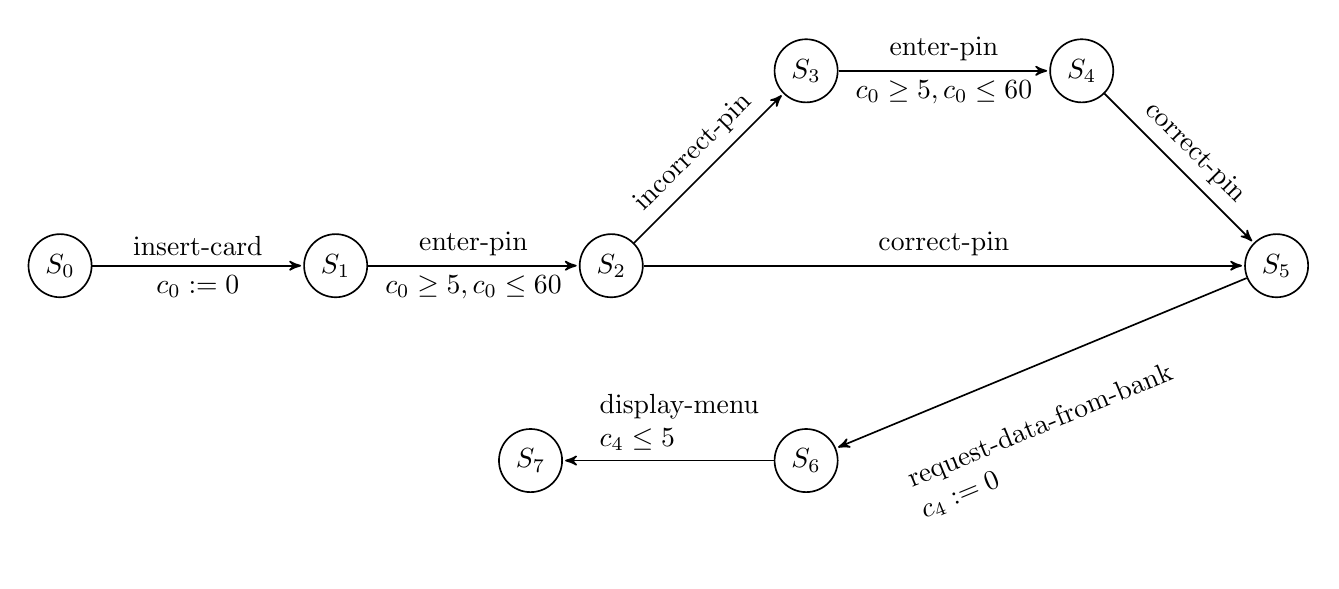
\begin{tikzpicture}[->,>=stealth',shorten >=0.8pt,auto,node distance=3.5cm,
		semithick]
		\tikzstyle{every state}=[draw,minimum size=1em]
		
		\node[state]         (S_0)              {$S_0$};
		\node[state]         (S_1) [right of=S_0] {$S_1$};
		\node[state]         (S_2) [right of=S_1] {$S_2$};
		\node[state]         (S_3) [above right of=S_2] {$S_3$};
		\node[state]         (S_4) [right of=S_3] {$S_4$};
		\node[state]         (S_5) [below right of=S_4] {$S_5$};
		\node[state]         (S_6) [below right of=S_2] {$S_6$};
		\node[state]         (S_7) [left of=S_6] {$S_7$}; 
		
		\path (S_0) edge                node[anchor=south, above]             {insert-card}           
		node[anchor=south, below]             {$c_0 := 0$}            (S_1)
		(S_1) edge                node[anchor=south, above]             {enter-pin} 
		node[anchor=north, below]             {$c_0\ge5,c_0\le60$}    (S_2)
		(S_2) edge                node[anchor=south, above,sloped]      {incorrect-pin}         (S_3)
		(S_3) edge                node[anchor=south, above]             {enter-pin} 
		node[anchor=north, below]             {$c_0\ge5,c_0\le60$}    (S_4)
		(S_4) edge                node[anchor=south, above,sloped]      {correct-pin}           (S_5)
		(S_2) edge                node[above]                           {correct-pin}           (S_5)
		(S_5) edge                node[anchor=north, below,sloped,text width=6cm]      {
			\centering
			\begin{itemize}
			\item[] request-data-from-bank\\$c_4 := 0$ 
			\end{itemize}
		}                       (S_6)
		(S_6) edge                node[anchor=south, above,text width=3.5cm] {
			\begin{itemize}
			\item[] display-menu\\$c_4\le5$
			\end{itemize}
		}                       (S_7)
		;
		\end{tikzpicture}
		\end{adjustbox}
		\caption{Timed automaton synthesized from Scenario 1 and Scenario 2}
		\label{fig:timedAutomaton}
	\end{figure}
\end{frame}

\begin{frame}{Automated Teller Machine (ATM)}
Explain extended scenario
\end{frame}

\begin{frame}{Automated Teller Machine (ATM)}
\begin{figure}
	\begin{adjustbox}{max totalsize={.99\textwidth}{.85\textheight},center}
		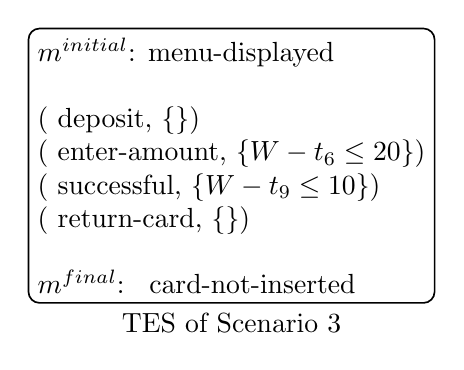
\begin{tikzpicture}[->,>=stealth']
		\tikzset{vertex/.style = {shape=rectangle,rounded corners, semithick, draw,align=left}}
		\node[vertex, label = below: TES of Scenario 3] (QUERY) 
		{ $m^{initial}$: {menu-displayed} \\
			\\
			({ deposit}, $\{\}$) \\
			({ enter-amount}, $\{W-t_6\leq 20\}$) \\
			({ successful}, $\{W-t_{9}\leq 10\}$) \\
			({ return-card}, $\{\}$) \\
			\\
			$m^{final}$: { card-not-inserted}
		};
		
		\end{tikzpicture}
	
		\hspace{0.5cm}
	
		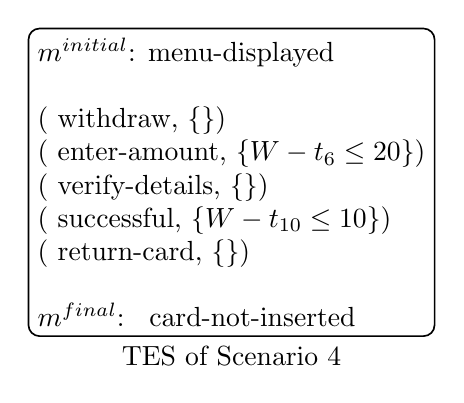
\begin{tikzpicture}[->,>=stealth']
		\tikzset{vertex/.style = {shape=rectangle,rounded corners, semithick, draw,align=left}}
		\node[vertex, label = below: TES of Scenario 4] (QUERY) 
		{ $m^{initial}$: {menu-displayed} \\
			\\
			({ withdraw}, $\{\}$) \\
			({ enter-amount}, $\{W-t_6\leq 20\}$) \\
			({ verify-details}, $\{\}$) \\
			({ successful}, $\{W-t_{10}\leq 10\}$) \\
			({ return-card}, $\{\}$) \\
			\\
			$m^{final}$: { card-not-inserted}
		};
		
		\end{tikzpicture}
		\end{adjustbox}
		\caption{Timed Event Sequences of the ATM with withdraw and deposit option}
		\label{fig:Timed Event Sequences of ATM with withdraw and deposit option}
	\end{figure}

\end{frame}

\begin{frame}{Automated Teller Machine (ATM)}
	\begin{figure}
		\begin{adjustbox}{max totalsize={.99\textwidth}{.85\textheight},center}			
			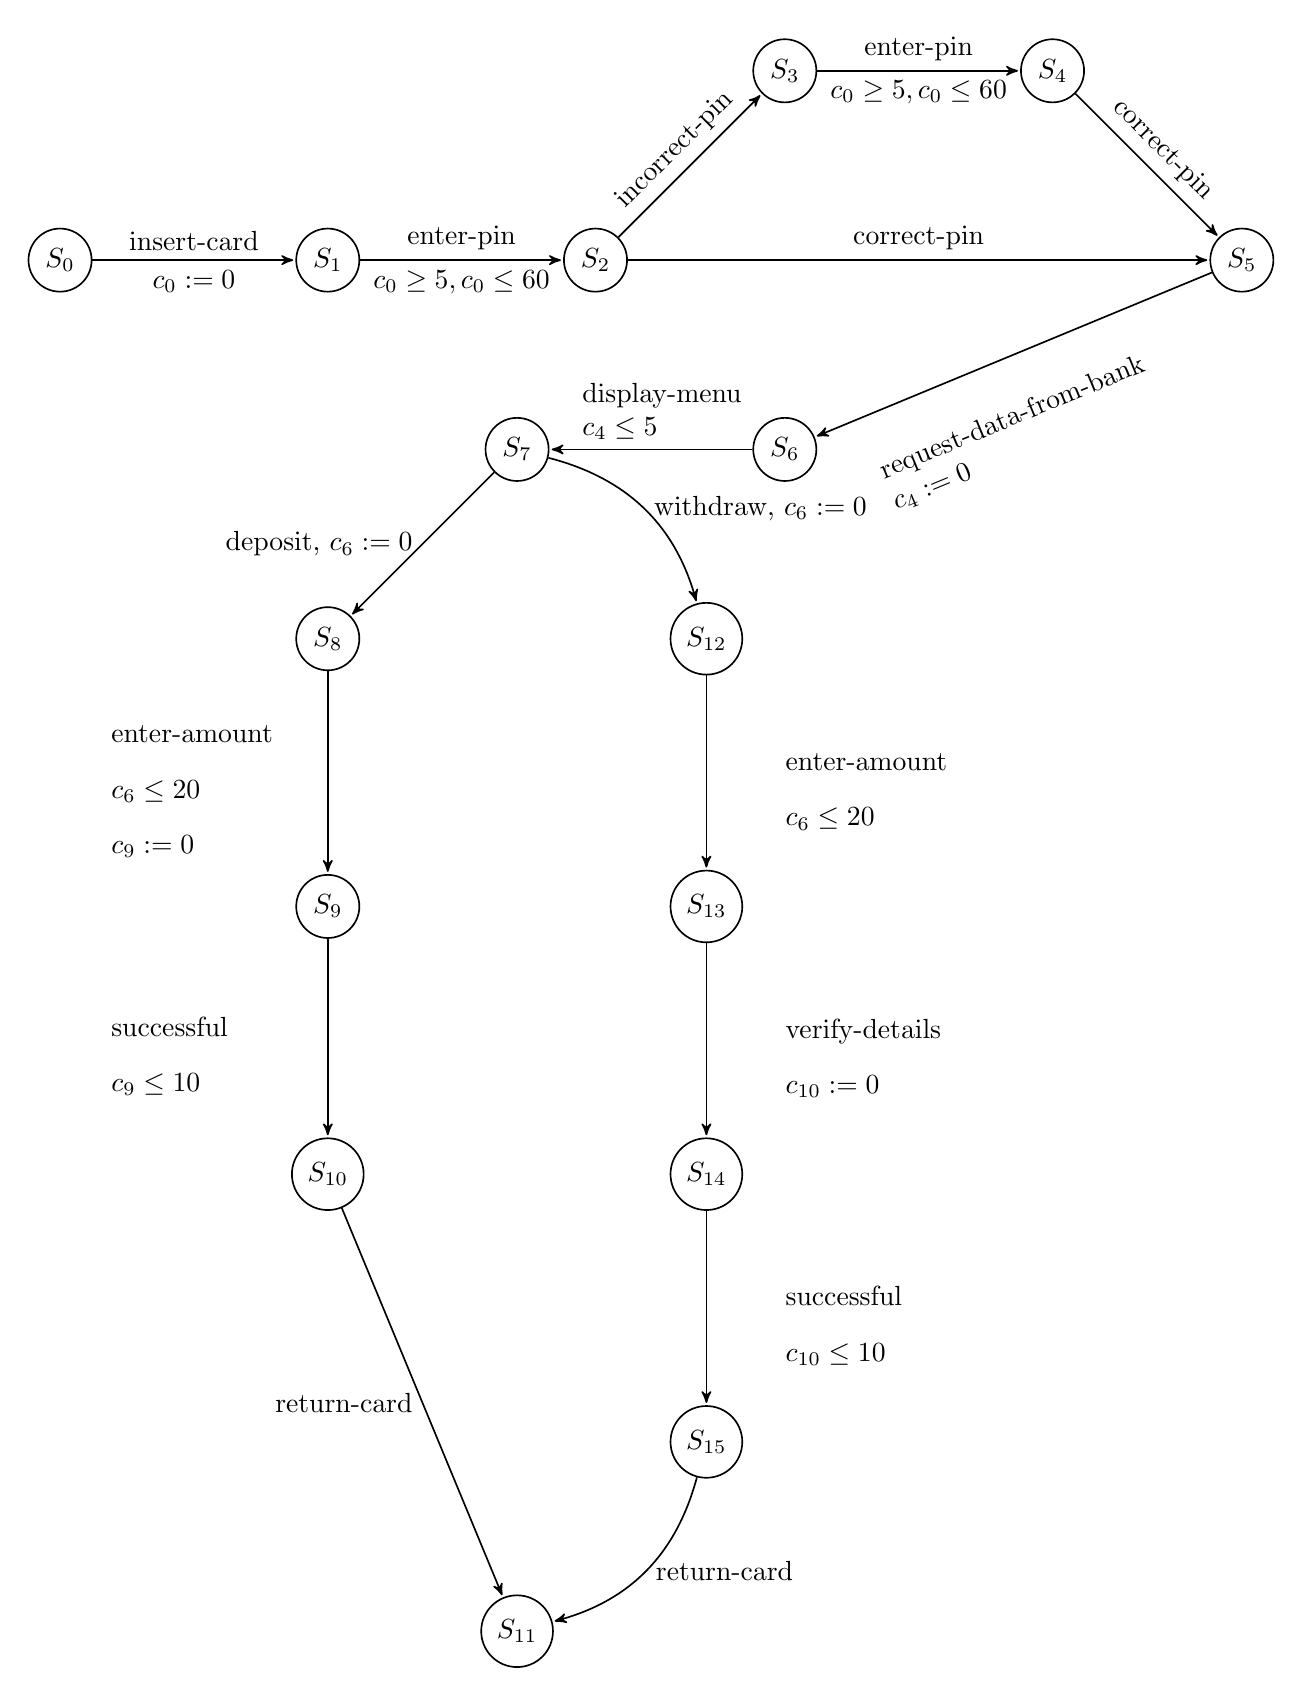
\begin{tikzpicture}[->,>=stealth',shorten >=0.8pt,auto,node distance=3.4cm,
			semithick]
			\tikzstyle{every state}=[draw,minimum size=1em]
			
			\node[state]         (S_0)              {$S_0$};
			\node[state]         (S_1) [right of=S_0] {$S_1$};
			\node[state]         (S_2) [right of=S_1] {$S_2$};
			\node[state]         (S_3) [above right of=S_2] {$S_3$};
			\node[state]         (S_4) [right of=S_3] {$S_4$};
			\node[state]         (S_5) [below right of=S_4] {$S_5$};
			\node[state]         (S_6) [below right of=S_2] {$S_6$};
			\node[state]         (S_7) [left of=S_6] {$S_7$};
			\node[state]         (S_8) [below left of=S_7] {$S_8$};
			
			\node[state]         (S_9) [below of=S_8] {$S_9$};
			\node[state]         (S_10) [below of=S_9] {$S_{10}$};
			
			\node[state]         (S_12) [below right of=S_7] {$S_{12}$};
			\node[state]         (S_13) [below of=S_12] {$S_{13}$};
			\node[state]         (S_14) [below of=S_13] {$S_{14}$};
			\node[state]         (S_15) [below of=S_14] {$S_{15}$};
			\node[state]         (S_11) [below left of=S_15] {$S_{11}$};
			
						
			\path (S_0) edge                node[anchor=south, above]             {insert-card}           
			node[anchor=south, below]             {$c_0 := 0$}            (S_1)
			(S_1) edge                node[anchor=south, above]             {enter-pin} 
			node[anchor=north, below]             {$c_0\ge5,c_0\le60$}    (S_2)
			(S_2) edge                node[anchor=south, above,sloped]      {incorrect-pin}         (S_3)
			(S_3) edge                node[anchor=south, above]             {enter-pin} 
			node[anchor=north, below]             {$c_0\ge5,c_0\le60$}    (S_4)
			(S_4) edge                node[anchor=south, above,sloped]      {correct-pin}           (S_5)
			(S_2) edge                node[above]                           {correct-pin}           (S_5)
			(S_5) edge                node[anchor=north, below,sloped,text width=6cm]      {
				\centering
				\begin{itemize}
				\item[] request-data-from-bank\\$c_4 := 0$ 
				\end{itemize}
			}                       (S_6)
			(S_6) edge                node[anchor=south, above,text width=3.5cm] 
			{ 
				\begin{itemize}
				\item[] display-menu\\$c_4\le5$
				\end{itemize}
			}                       (S_7)
			(S_7) edge                node[left]                            {deposit, $c_6:=0$}               (S_8)
			
			(S_8) edge                node[anchor=right, left,text width=3.5cm] 
			{ 
				\begin{itemize}
				\item[] enter-amount
				\item[] $c_6\le20$
				\item[] $c_9:=0$
				\end{itemize}
			}                        (S_9)
			(S_9) edge                node[anchor=right, left,text width=3.5cm] 
			{ 
				\begin{itemize}
				\item[] successful
				\item[] $c_{9}\le10$
				\end{itemize}
			}                       (S_10)
			(S_10) edge               node[left]                            {return-card}           (S_11)
			
			(S_7) edge   [bend left]  node[right]                           {withdraw, $c_6:=0$}              (S_12)
			(S_12) edge               node[anchor=left, right,text width=3.5cm] 
			{ 
				\begin{itemize}
				\item[] enter-amount
				\item[] $c_6\le20$
				\end{itemize}
			}                       (S_13)
			(S_13) edge               node[anchor=left, right,text width=3.5cm] 
			{ 
				\begin{itemize}
				\item[] verify-details
				\item[] $c_{10}:= 0$
				\end{itemize}
			}                       (S_14)
			(S_14) edge               node[anchor=left, right,text width=3.5cm] 
			{ 
				\begin{itemize}
				\item[] successful
				\item[] $c_{10}\le10$
				\end{itemize}
			}                       (S_15)
			(S_15) edge  [bend left]  node[right]                           {return-card}           (S_11)
			;
			\end{tikzpicture}
		\end{adjustbox}
		\caption{The synthesized timed automaton of the ATM}
		\label{fig:Synthesized ATM TA}
	\end{figure}
\end{frame}


\begin{frame}{Light Control System}
	\begin{figure}[!ht]
		\begin{center}
%			\begin{minipage}{0.8\textwidth}
				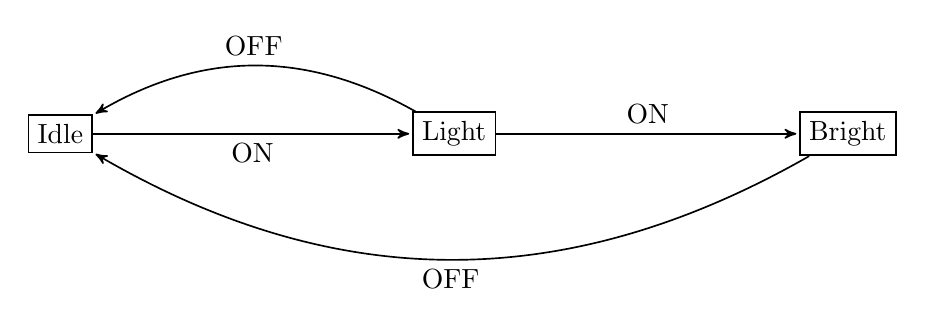
\begin{tikzpicture}[->,>=stealth',shorten >=1pt,auto,node distance=5cm,
				semithick]
				\tikzstyle{every state}=[shape=rectangle,draw,minimum size=1em]
				
				\node[state]       (Idle)                    {Idle};
				\node[state]       (Light)  [right of=Idle]     {Light};
				\node[state]       (Bright) [right of=Light]     {Bright};
				
				\path (Idle) edge                   node[below]  {ON}  (Light)
				(Light) edge    [bend right]  node[above]  {OFF}  (Idle)
				(Light) edge                  node[above]  {ON}  (Bright)
				(Bright) edge   [bend left]   node[below]  {OFF}  (Idle)    
				;
				\end{tikzpicture}
%			\end{minipage}
		\end{center}
		\caption{Mode graph of the Light Control System}
		\label{fig:MG_Light Control System}
		\vspace{0.1cm}
	\end{figure}
\end{frame}

\begin{frame}{Light Control System}
		\begin{figure}
			\begin{adjustbox}{max totalsize={.99\textwidth}{.85\textheight},center}
	
%			\begin{minipage}[b]{.25\textwidth}
				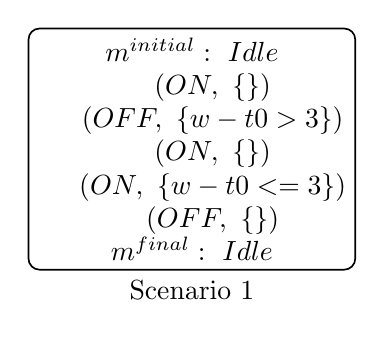
\begin{tikzpicture}[->,>=stealth']
				\tikzset{vertex/.style = {shape=rectangle,rounded corners, semithick, draw,align=center}}
				\node[vertex, label = below: Scenario 1] (QUERY) 
				{$m^{initial}:~Idle$ \\                                
					\indent    ($ON,~\{\}$) \\
					\indent    ($OFF, ~\{w-t0 > 3\}$) \\
					\indent    ($ON,~\{\}$) \\
					\indent    ($ON, ~\{w-t0 <= 3\}$) \\
					\indent    ($OFF,~\{\}$) \\                
					$m^{final}:~Idle$};
				
				\end{tikzpicture}
%			\end{minipage}
			\hspace{0.5cm}
%			\begin{minipage}[b]{.25\textwidth}
				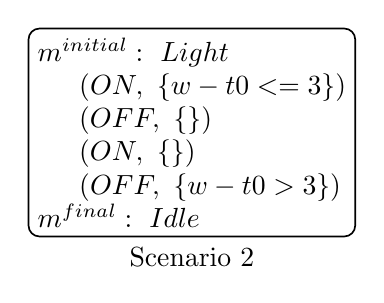
\begin{tikzpicture}[->,>=stealth']
				\tikzset{vertex/.style = {shape=rectangle,rounded corners, semithick, draw,align=left}}
				\node[vertex, label = below: Scenario 2] (QUERY) 
				{$m^{initial}:~Light$ \\
					
					\indent    ($ON,~\{w-t0 <= 3\}$) \\
					\indent    ($OFF,~\{\}$) \\
					\indent    ($ON,~\{\}$) \\
					\indent    ($OFF,~\{w-t0 > 3\}$) \\
					
					$m^{final}:~Idle$};
				
				\end{tikzpicture}
%			\end{minipage}
			\hspace{0.5cm}
%			\begin{minipage}[b]{.25\textwidth}
				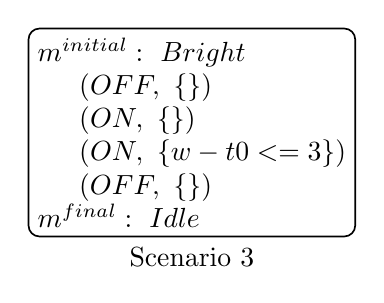
\begin{tikzpicture}[->,>=stealth']
				\tikzset{vertex/.style = {shape=rectangle,rounded corners, semithick, draw,align=left}}
				\node[vertex, label = below: Scenario 3] (QUERY) 
				{$m^{initial}:~Bright$ \\
					
					\indent    ($OFF,~\{\}$) \\
					\indent    ($ON,~\{\}$) \\
					\indent    ($ON,~\{w-t0 <= 3\}$) \\
					\indent    ($OFF,~\{\}$) \\
					
					$m^{final}:~Idle$};
				
				\end{tikzpicture}
%			\end{minipage}
		
		\end{adjustbox}
		\caption{Timed Event Sequences of the Light Control System}
		\label{fig:Timed Event Sequences of Light Control System}
	\end{figure}
\end{frame}

\begin{frame}{Light Control System}
	\begin{figure}
		\begin{adjustbox}{max totalsize={.99\textwidth}{.8\textheight},center}
			\begin{tikzpicture}[->,>=stealth',shorten >=1pt,auto,node distance=2.3cm,
			semithick]
			\tikzstyle{every state}=[draw,minimum size=1.65cm]
			
			\node[state]         (S_0) [yshift=-1.5cm]                   {$Idle$};
			\node[state]         (S_1) [below of=S_0,yshift=-1cm]     {$Light$};
			\node[state]         (S_2) [below of=S_1,yshift=-1cm]     {$Idle$};
			\node[state]         (S_3) [below of=S_2,yshift=-1cm]     {$Light$};
			\node[state]         (S_4) [below of=S_3,yshift=-1cm]   {$Bright$};
			\node[state]         (S_5) [right of=S_4,xshift=1cm]    {$Idle$};
			\node[state]         (S_6) [right of=S_5,xshift=1.6cm]    {$Light$};
			\node[state]         (S_7) [right of=S_6,xshift=1.6cm]    {$Idle$};
			\node[state]         (S_8) [above right of=S_6,xshift=1cm,yshift=1cm]    {$Bright$};
			
			\path (S_0) edge              node[right]  {ON [$c_0 := 0$]}  (S_1)
			(S_1) edge              node[right]  {OFF [$c_0 > 3$]}  (S_2)
			(S_2) edge              node[right]  {ON [$c_0 := 0$]}  (S_3)
			(S_1) edge [bend right] node[left]   {ON [$c_0 <= 3$]}  (S_4)
			(S_3) edge              node[right]  {ON [$c_0 <= 3$]}  (S_4)
			(S_4) edge              node[below]  {OFF}  (S_5)
			(S_5) edge              node[below]  {ON [$c_0 := 0$]}  (S_6)
			(S_6) edge              node[below]  {OFF [$c_0 > 3$]}  (S_7)
			(S_6) edge [bend left]  node[left]   {ON [$c_0 <= 3$]}  (S_8)
			(S_8) edge [bend left]  node[right]  {OFF}  (S_7)
			
			;
			\end{tikzpicture}
		\end{adjustbox}
	
		\caption{Timed automaton of the Light Control System}
		\label{fig:TA_Ligt Control System}
	\end{figure}
\end{frame}

\begin{frame}{Traffic Light}
	\begin{figure}
		\begin{adjustbox}{max totalsize={.99\textwidth}{.8\textheight},center}
		
		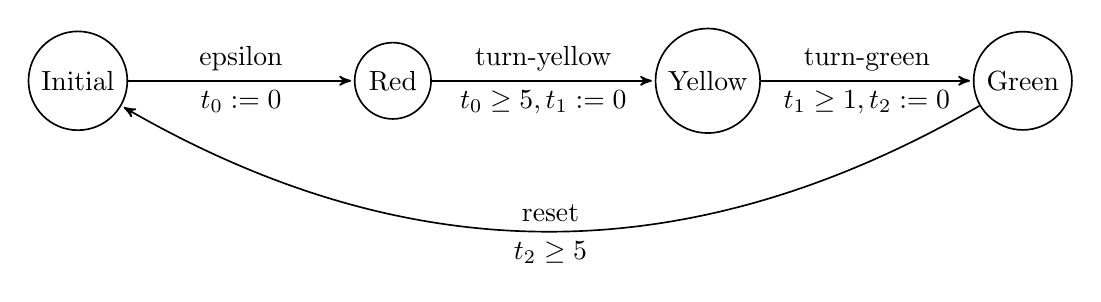
\begin{tikzpicture}[->,>=stealth',shorten >=1pt,auto,node distance=4cm,
		semithick]
		\tikzstyle{every state}=[draw,minimum size=1em]
		
		\node[state]       (Initial)                        {Initial};
		\node[state]       (Red)      [right of=Initial]    {Red};
		\node[state]       (Yellow)   [right of=Red]        {Yellow};
		\node[state]       (Green)    [right of=Yellow]      {Green};
		
		
		\path (Initial)   edge          node[anchor=south, above] {epsilon} 
		node[anchor=north, below] {$t_0:=0$}       (Red)
		(Red)       edge                 node[anchor=south, above] {turn-yellow}
		node[anchor=north, below] {$t_0\ge5,t_1:=0$}     (Yellow)
		(Yellow)    edge                 node[anchor=south, above] {turn-green} 
		node[anchor=north, below] {$t_1\ge1,t_2:=0$}     (Green)
		(Green)     edge   [bend left]   node[anchor=south, above] {reset} 
		node[anchor=north, below] {$t_2\ge5$}           (Initial)   
		;
		\end{tikzpicture}
		\end{adjustbox}
		\caption{Timed automaton of the Traffic Light}
		\label{fig:TrafficLight}		
	\end{figure}
\end{frame}

\begin{frame}{Traffic Light}
	\begin{figure}
		\begin{adjustbox}{max totalsize={.99\textwidth}{.8\textheight},center}		
	
		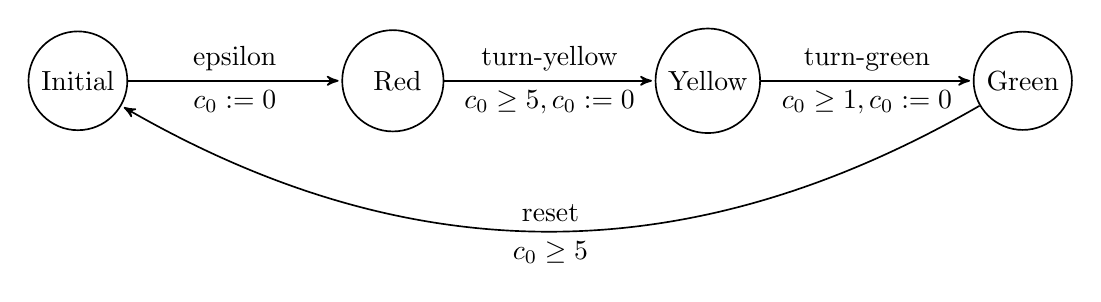
\begin{tikzpicture}[->,>=stealth',shorten >=1pt,auto,node distance=4cm,
		semithick]
		\tikzstyle{every state}=[draw,minimum size=1em]
		
		\node[state]       (Initial)                        {Initial};
		\node[state]       (Red)      [right of=Initial]    {~~Red~~};
		\node[state]       (Yellow)   [right of=Red]        {Yellow};
		\node[state]       (Green)    [right of=Yellow]      {Green};
		
		
		\path (Initial)   edge          node[anchor=south, above] {epsilon} 
		node[anchor=north, below] {$c_0:=0$}       (Red)
		(Red)       edge                 node[anchor=south, above] {turn-yellow}
		node[anchor=north, below] {$c_0\ge5,c_0:=0$}     (Yellow)
		(Yellow)    edge                 node[anchor=south, above] {turn-green} 
		node[anchor=north, below] {$c_0\ge1,c_0:=0$}     (Green)
		(Green)     edge   [bend left]   node[anchor=south, above] {reset} 
		node[anchor=north, below] {$c_0\ge5$}           (Initial)   
		;
		\end{tikzpicture}
	
		\end{adjustbox}
		\caption{The optimally allocated timed automaton of the Traffic Light}
		\label{fig:OptimalTrafficLight}
	\end{figure}
\end{frame}

\begin{frame}{CSMA/CD Protocol}
	\begin{figure}
		\begin{adjustbox}{max totalsize={.99\textwidth}{.8\textheight},center}	
			\begin{tikzpicture}[->,>=stealth',shorten >=1pt,auto,node distance=8cm,
			semithick]
			\tikzstyle{every state}=[draw,minimum size=2cm]
			
			\node[state]         (init)                    {$init$};
			\node[state]         (send) [right of=init]  {$send$};
			\node[state]         (cd_1) [below right of=send]  {$cd_1$};
			\node[state]         (transm) [left of=cd_1] {$transm$};
			\node[state]         (cd_2) [below of=transm]  {$cd_2$};
			
			
			\path (init) edge                   node[below] {r1  [$x_0:=0$]}  (send)
			(init) edge   [bend left]     node[above] {r11 [$x_0:=0$]}  (send)
			(init) edge   [loop above]    node[]      {r10}  (init)
			(send) edge   [bend right]    node[sloped,anchor=center,below,text width=4cm]  {r2  [$x_0=0,x_1:=0$]}  (cd_1)
			(send) edge                   node[sloped,anchor=center,below,text width=4cm]  {r3  [$x_0=0,x_1:=0$]}  (cd_1)
			(send) edge                   node[sloped,anchor=center,above,text width=4cm]  {r5  [$x_0=0,x_1:=0$]}  (transm)
			(cd_1) edge   [bend right]    node[sloped,anchor=center,above,text width=3cm] {r4  [$x_1<=2\sigma$]}  (send)
			(cd_1) edge   [loop below]    node[]      {r9}  (cd_1)
			(transm) edge                 node[sloped,anchor=center,above,text width=2cm]  {r6  [$x_1=\lambda$]}  (init)
			(transm) edge [bend left]     node[right]  {r7  [$x_1<=\lambda,x_3:=0$]}  (cd_2)
			(cd_2) edge   [bend  left]    node[sloped,anchor=center,above,text width=3cm]  {r8  [$x_3<=2\lambda$]}  (init)
			
			;
			\end{tikzpicture}
		\end{adjustbox}
		\caption{The timed automaton for the sender in CSMA/CD protocol}
		\label{fig:CSMA/CD}
	\end{figure}
\end{frame}


\begin{frame}{CSMA/CD Protocol}
	\begin{figure}
		\begin{adjustbox}{max totalsize={.99\textwidth}{.8\textheight},center}	

		\begin{tikzpicture}[->,>=stealth',shorten >=1pt,auto,node distance=8cm,
		semithick]
		\tikzstyle{every state}=[draw,minimum size=2cm]
		
		\node[state]         (init)                    {$init$};
		\node[state]         (send) [right of=init]  {$send$};
		\node[state]         (cd_1) [below right of=send]  {$cd_1$};
		\node[state]         (transm) [left of=cd_1] {$transm$};
		\node[state]         (cd_2) [below of=transm]  {$cd_2$};
		
		
		\path (init) edge                   node[below]                                      {r1  [$c_1:=0$]}  (send)
		(init) edge   [bend left]     node[above]                                      {r11 [$c_1:=0$]}  (send)
		(init) edge   [loop above]    node[]                                           {r10}             (init)
		(send) edge   [bend right]    node[sloped,anchor=center,below,text width=4cm]  {r2  [$c_1=0,c_2:=0$]}  (cd_1)
		(send) edge                   node[sloped,anchor=center,below,text width=4cm]  {r3  [$c_1=0,c_2:=0$]}  (cd_1)
		(send) edge                   node[sloped,anchor=center,above,text width=4cm]  {r5  [$c_1=0,c_2:=0$]}  (transm)
		(cd_1) edge   [bend right]    node[sloped,anchor=center,above,text width=3cm]  {r4  [$c_2<=2\sigma$]}  (send)
		(cd_1) edge   [loop below]    node[]                                           {r9}                    (cd_1)
		(transm) edge                 node[sloped,anchor=center,above,text width=2cm]  {r6  [$c_1=\lambda$]}  (init)
		(transm) edge [bend left]     node[right]                                      {r7  [$c_1<=\lambda,c_1:=0$]}  (cd_2)
		(cd_2) edge   [bend  left]    node[sloped,anchor=center,above,text width=3cm]  {r8  [$c_1<=2\lambda$]}  (init)
		
		;
		\end{tikzpicture}
		\end{adjustbox}
		\caption{The optimally allocated timed automaton for the sender in CSMA/CD protocol}
		\label{fig:OptimalCSMA/CD}
	\end{figure}
\end{frame}

\section{Conclusion}

\begin{frame}{Conclusion}
	conclude here
	\cite{FromScenariosToTimedAutomata-2016}
	\cite{OptimalClockAllocationTA}
\end{frame}

\begin{frame}[standout]
THANK PROFESSORS???
Neda and Committee mem??
\end{frame}
\begin{frame}[standout]
	Questions?
\end{frame}


\begin{frame}[allowframebreaks]{References}
	\bibliography{ResearchPPT}
	\bibliographystyle{abbrv}
\end{frame}

\end{document}